% =============================================================================
% 04-expression-evaluation-notes.tex — Lecture Notes for Week 4:
% Why Compilers Rewrite Your Arithmetic (Conversion, Hanoi, and Recursion
% with the Runtime Stack)
%
% DERIVED ARTIFACT. Source of truth: Slides/CS301/04-expression-evaluation.tex
% (41 frames/41 pages, compiled clean).
% Generated by /lecture-notes at the "textbook-candidate prose" Detail Bar
% (every trace step written out, every example fully solved, Exercises with a
% separate Solutions block, reading guidance per section); do not hand-edit
% content independently of the Beamer source without re-running /qa-notes
% afterward (single-source-of-truth.md).
%
% Page-grounding (inherited 1:1 from the deck header; no upgrades):
%   Karumanchi2017 Ch.4 (Stacks, pp.163-204 PDF: infix/postfix/prefix
%     applications) and Ch.2 (pp.62-73 PDF: recursion, call stack,
%     recursion vs iteration); Wirth Ch.3 (pp.87-108: recursive algorithms,
%     when recursion helps and when it does not); Sedgewick2011 p.120 (stack
%     as a collection ADT, deck-header context only); Horowitz & Sahni Ch.3 /
%     Aho-Hopcroft-Ullman Ch.2 at chapter level only (not page-indexed).
%   Socratic "Check Your Prediction" frames and the three "Before You Go"
%   predictions are folded into the prose as worked checks with the deck's
%   own answers; the Week 5 (queues) and Week 11 (expression trees) forward
%   pointers are preserved as stated.
%
% Compile with (Windows/MiKTeX, ';'-joined TEXINPUTS/BIBINPUTS): cd Notes/CS301 &&
%   $env:TEXINPUTS="../../Preambles;"; xelatex -interaction=nonstopmode 04-expression-evaluation-notes.tex
%   $env:BIBINPUTS="../..;"; bibtex 04-expression-evaluation-notes
%   $env:TEXINPUTS="../../Preambles;"; xelatex -interaction=nonstopmode 04-expression-evaluation-notes.tex  (x2)
% =============================================================================

\documentclass[11pt]{article}
\usepackage[margin=1in]{geometry}
% =============================================================================
% Preambles/header.tex — shared LaTeX/Beamer preamble for this project
%
% Use from a Beamer lecture by prepending:
%     % =============================================================================
% Preambles/header.tex — shared LaTeX/Beamer preamble for this project
%
% Use from a Beamer lecture by prepending:
%     % =============================================================================
% Preambles/header.tex — shared LaTeX/Beamer preamble for this project
%
% Use from a Beamer lecture by prepending:
%     \input{header}
% and compiling with TEXINPUTS=../Preambles:$TEXINPUTS (the /compile-latex
% skill does this automatically).
%
% PALETTE CONTRACT. Color names defined here MUST match the names in
% Quarto/theme-template.scss so Beamer and Quarto renderings use the same
% palette. The scripts/check-palette-sync.sh script enforces this.
%
% To customize: edit the HEX values below AND the matching $variable in
% Quarto/theme-template.scss, then run scripts/check-palette-sync.sh.
%
% TITLE PAGE. A formal, serif (Libertine) title-page template is defined in
% the Beamer-only block below (\setbeamertemplate{title page}) -- title,
% subtitle, a thin gold rule, then \author/\institute/\date. Frametitle and
% body text remain on Beamer's sans-serif default. No SCSS counterpart is
% needed for this (font/layout only, no new colors).
% =============================================================================

% -----------------------------------------------------------------------------
% Engine detection + encoding
%
% Our /compile-latex skill uses XeLaTeX, where inputenc is unnecessary and
% can produce encoding warnings. Only load inputenc under pdfTeX.
% -----------------------------------------------------------------------------
\usepackage{iftex}
\ifPDFTeX
  \usepackage[utf8]{inputenc}
\fi

\usepackage{amsmath, amssymb, amsthm}
\usepackage{booktabs}
\usepackage{graphicx}

% -----------------------------------------------------------------------------
% Serif face for the title page (formal/academic look). Linux Libertine is
% XeLaTeX- and pdfTeX-safe and redefines \rmdefault, so \rmfamily picks it up
% everywhere \rmfamily is used explicitly. Body text and frametitles stay on
% Beamer's own sans-serif default (unaffected) -- only the title-page
% \setbeamerfont{...} overrides below opt in to \rmfamily.
% -----------------------------------------------------------------------------
\usepackage{libertine}

% -----------------------------------------------------------------------------
% PALETTE — mirrors Quarto/theme-template.scss variable names.
% Load xcolor and define colors BEFORE anything that references them
% (notably hyperref, hypersetup, and the Beamer color assignments).
% -----------------------------------------------------------------------------
\usepackage{xcolor}

\definecolor{primary-blue}{HTML}{012169}      % headings, accents
\definecolor{primary-gold}{HTML}{B9975B}      % emphasis, borders
\definecolor{highlight-yellow}{HTML}{F2A900}  % markers, alerts
\definecolor{light-bg}{HTML}{E8EDF5}          % title / section backgrounds
\definecolor{jet}{HTML}{1A1A1A}               % body text

% Semantic colors (used in diagrams and annotations)
\definecolor{positive}{HTML}{15803D}          % good / observed / identified
\definecolor{negative}{HTML}{B91C1C}          % bad / problematic / bias
\definecolor{neutral}{HTML}{525252}           % reference / context

% Highlight accents (match .hi-* classes in the SCSS)
\definecolor{hi-slate}{HTML}{314F4F}
\definecolor{hi-green}{HTML}{2E8B57}
\definecolor{hi-red}{HTML}{C41E3A}

% Semantic aliases so skill templates and snippets can write
% \textcolor{accent}{...} without hard-coding "primary-blue".
\colorlet{accent}{primary-blue}
\colorlet{accent2}{primary-gold}

% -----------------------------------------------------------------------------
% Hyperref — loaded AFTER xcolor + palette so link colors resolve.
% -----------------------------------------------------------------------------
\usepackage{hyperref}
\hypersetup{colorlinks=true, linkcolor=primary-blue, urlcolor=primary-blue,
            citecolor=primary-blue, pdfborder={0 0 0}}

% -----------------------------------------------------------------------------
% Course code — set once per deck (after \input{header}, before \begin{document})
% via \coursecode{CS401}. Shown in the footer on every slide so a deck's course
% is identifiable without opening the title page. Empty by default.
% -----------------------------------------------------------------------------
\makeatletter
\newcommand{\coursecode}[1]{\gdef\@coursecodetext{#1}}
\gdef\@coursecodetext{}
\makeatother

% -----------------------------------------------------------------------------
% Beamer theme assignments (only apply under Beamer).
%
% We detect Beamer via \@ifclassloaded{beamer}, which is the documented,
% non-internal way. This must be wrapped in \makeatletter/\makeatother
% because \@ifclassloaded contains an @-catcode character.
% -----------------------------------------------------------------------------
\makeatletter
\@ifclassloaded{beamer}{%
  \usefonttheme{professionalfonts}
  \setbeamercolor{structure}{fg=primary-blue}
  \setbeamercolor{frametitle}{fg=primary-blue}
  \setbeamercolor{title}{fg=primary-blue}
  \setbeamercolor{subtitle}{fg=primary-gold}
  \setbeamercolor{author}{fg=primary-blue}
  \setbeamercolor{institute}{fg=neutral}
  \setbeamercolor{date}{fg=primary-gold}
  \setbeamercolor{itemize item}{fg=primary-blue}
  \setbeamercolor{itemize subitem}{fg=primary-gold}
  \setbeamercolor{alerted text}{fg=primary-gold}
  \setbeamercolor{block title}{fg=white, bg=primary-blue}
  \setbeamercolor{block body}{bg=light-bg}
  % Semantic block variants: block=definition/concept (blue), exampleblock=
  % worked example (green/positive), alertblock=key takeaway or caution (gold).
  % Keep to <=2 colored boxes per slide across ALL three variants (INV-7).
  \setbeamercolor{block title example}{fg=white, bg=positive}
  \setbeamercolor{block body example}{bg=light-bg}
  \setbeamercolor{block title alerted}{fg=white, bg=primary-gold}
  \setbeamercolor{block body alerted}{bg=light-bg}

  % ---------------------------------------------------------------------------
  % Formal title page: serif (Libertine, via \rmfamily) for title-page
  % elements only. Body text, itemize, and frametitle are intentionally left
  % on Beamer's sans-serif default -- \usebeamerfont{title} is also what
  % \transitionslide (below) uses for its big centered text, so section
  % transitions pick up the same serif treatment for free.
  % ---------------------------------------------------------------------------
  \setbeamerfont{title}{family=\rmfamily, series=\bfseries, size=\Large}
  \setbeamerfont{subtitle}{family=\rmfamily, shape=\itshape, size=\normalsize}
  \setbeamerfont{author}{family=\rmfamily, size=\normalsize}
  \setbeamerfont{institute}{family=\rmfamily, size=\scriptsize}
  \setbeamerfont{date}{family=\rmfamily, size=\scriptsize}

  \setbeamertemplate{title page}{
    \vfill
    \begin{center}
      {\usebeamerfont{title}\usebeamercolor[fg]{title}\inserttitle\par}
      \vspace{0.15cm}
      {\usebeamerfont{subtitle}\usebeamercolor[fg]{subtitle}\insertsubtitle\par}
      \vspace{0.45cm}
      {\color{primary-gold}\rule{0.42\textwidth}{0.6pt}\par}
      \vspace{0.45cm}
      {\usebeamerfont{author}\usebeamercolor[fg]{author}\insertauthor\par}
      \vspace{0.35cm}
      {\usebeamerfont{institute}\usebeamercolor[fg]{institute}\insertinstitute\par}
      \vspace{0.35cm}
      {\usebeamerfont{date}\usebeamercolor[fg]{date}\insertdate\par}
    \end{center}
    \vfill
  }

  % Minimal footer: course code (left) + page X / N (right), no navigation clutter
  \setbeamertemplate{navigation symbols}{}
  \setbeamertemplate{footline}{%
    \color{neutral}\footnotesize\hspace{0.7em}\@coursecodetext\hfill
    \insertframenumber/\inserttotalframenumber\hspace{0.7em}\vspace{0.3em}}
}{}
\makeatother

% -----------------------------------------------------------------------------
% TikZ setup — libraries the snippet gallery uses
% -----------------------------------------------------------------------------
\usepackage{tikz}
\usetikzlibrary{arrows.meta, positioning, calc, decorations.pathreplacing,
                fit, shapes.geometric, backgrounds}

% Shared TikZ styles — snippets and hand-written diagrams can pick these up
% via `\begin{tikzpicture}[every node/.style={...}]` or by naming specific
% styles (e.g., `\node[dag-node] (X) at (0,0) {X};`).
\tikzset{
  % Node styles for causal DAGs and similar
  dag-node/.style = {
    draw=primary-blue, fill=light-bg, rounded corners=2pt,
    minimum width=1.2cm, minimum height=0.9cm, align=center, font=\small
  },
  decision-node/.style = {
    draw=primary-gold, fill=white, diamond, aspect=1.8,
    minimum width=1.8cm, minimum height=1.2cm, align=center, font=\small,
    inner sep=1pt
  },
  % Edge styles — observed vs counterfactual
  observed-edge/.style = {-{Latex[length=2.5mm]}, thick, draw=jet},
  counterfactual-edge/.style = {-{Latex[length=2.5mm]}, thick, draw=neutral, dashed},
  confound-edge/.style = {-{Latex[length=2.5mm]}, thick, draw=negative, dashed},
  % Data-point styles for plots
  observed-dot/.style = {fill=primary-blue, draw=primary-blue, circle, inner sep=1.2pt},
  counterfactual-dot/.style = {fill=white, draw=neutral, circle, inner sep=1.2pt}
}

% -----------------------------------------------------------------------------
% Convenience macros
% -----------------------------------------------------------------------------
\newcommand{\muted}[1]{\textcolor{neutral}{#1}}
\newcommand{\key}[1]{\textcolor{primary-gold}{\textbf{#1}}}
\newcommand{\good}[1]{\textcolor{positive}{#1}}
\newcommand{\bad}[1]{\textcolor{negative}{#1}}

% Standout frame macro: full-bleed dark background for section transitions.
% Beamer-only (uses \begin{frame}/\setbeamercolor/\usebeamerfont) -- do not
% call from an article-class file (e.g. Notes/<CODE>/*-notes.tex). \muted,
% \key, \good, \bad, and \coursecode above are plain xcolor/gdef and are
% safe to use from either class; verified when Notes/article-class support
% was added.
% Expand: \transitionslide{Your transition title}
\newcommand{\transitionslide}[1]{%
  \begingroup
  \setbeamercolor{background canvas}{bg=primary-blue}
  \begin{frame}[plain]
    \centering
    \vfill
    {\usebeamerfont{title}\color{white}\Large #1\par}
    \vfill
  \end{frame}
  \endgroup
}

% and compiling with TEXINPUTS=../Preambles:$TEXINPUTS (the /compile-latex
% skill does this automatically).
%
% PALETTE CONTRACT. Color names defined here MUST match the names in
% Quarto/theme-template.scss so Beamer and Quarto renderings use the same
% palette. The scripts/check-palette-sync.sh script enforces this.
%
% To customize: edit the HEX values below AND the matching $variable in
% Quarto/theme-template.scss, then run scripts/check-palette-sync.sh.
%
% TITLE PAGE. A formal, serif (Libertine) title-page template is defined in
% the Beamer-only block below (\setbeamertemplate{title page}) -- title,
% subtitle, a thin gold rule, then \author/\institute/\date. Frametitle and
% body text remain on Beamer's sans-serif default. No SCSS counterpart is
% needed for this (font/layout only, no new colors).
% =============================================================================

% -----------------------------------------------------------------------------
% Engine detection + encoding
%
% Our /compile-latex skill uses XeLaTeX, where inputenc is unnecessary and
% can produce encoding warnings. Only load inputenc under pdfTeX.
% -----------------------------------------------------------------------------
\usepackage{iftex}
\ifPDFTeX
  \usepackage[utf8]{inputenc}
\fi

\usepackage{amsmath, amssymb, amsthm}
\usepackage{booktabs}
\usepackage{graphicx}

% -----------------------------------------------------------------------------
% Serif face for the title page (formal/academic look). Linux Libertine is
% XeLaTeX- and pdfTeX-safe and redefines \rmdefault, so \rmfamily picks it up
% everywhere \rmfamily is used explicitly. Body text and frametitles stay on
% Beamer's own sans-serif default (unaffected) -- only the title-page
% \setbeamerfont{...} overrides below opt in to \rmfamily.
% -----------------------------------------------------------------------------
\usepackage{libertine}

% -----------------------------------------------------------------------------
% PALETTE — mirrors Quarto/theme-template.scss variable names.
% Load xcolor and define colors BEFORE anything that references them
% (notably hyperref, hypersetup, and the Beamer color assignments).
% -----------------------------------------------------------------------------
\usepackage{xcolor}

\definecolor{primary-blue}{HTML}{012169}      % headings, accents
\definecolor{primary-gold}{HTML}{B9975B}      % emphasis, borders
\definecolor{highlight-yellow}{HTML}{F2A900}  % markers, alerts
\definecolor{light-bg}{HTML}{E8EDF5}          % title / section backgrounds
\definecolor{jet}{HTML}{1A1A1A}               % body text

% Semantic colors (used in diagrams and annotations)
\definecolor{positive}{HTML}{15803D}          % good / observed / identified
\definecolor{negative}{HTML}{B91C1C}          % bad / problematic / bias
\definecolor{neutral}{HTML}{525252}           % reference / context

% Highlight accents (match .hi-* classes in the SCSS)
\definecolor{hi-slate}{HTML}{314F4F}
\definecolor{hi-green}{HTML}{2E8B57}
\definecolor{hi-red}{HTML}{C41E3A}

% Semantic aliases so skill templates and snippets can write
% \textcolor{accent}{...} without hard-coding "primary-blue".
\colorlet{accent}{primary-blue}
\colorlet{accent2}{primary-gold}

% -----------------------------------------------------------------------------
% Hyperref — loaded AFTER xcolor + palette so link colors resolve.
% -----------------------------------------------------------------------------
\usepackage{hyperref}
\hypersetup{colorlinks=true, linkcolor=primary-blue, urlcolor=primary-blue,
            citecolor=primary-blue, pdfborder={0 0 0}}

% -----------------------------------------------------------------------------
% Course code — set once per deck (after % =============================================================================
% Preambles/header.tex — shared LaTeX/Beamer preamble for this project
%
% Use from a Beamer lecture by prepending:
%     \input{header}
% and compiling with TEXINPUTS=../Preambles:$TEXINPUTS (the /compile-latex
% skill does this automatically).
%
% PALETTE CONTRACT. Color names defined here MUST match the names in
% Quarto/theme-template.scss so Beamer and Quarto renderings use the same
% palette. The scripts/check-palette-sync.sh script enforces this.
%
% To customize: edit the HEX values below AND the matching $variable in
% Quarto/theme-template.scss, then run scripts/check-palette-sync.sh.
%
% TITLE PAGE. A formal, serif (Libertine) title-page template is defined in
% the Beamer-only block below (\setbeamertemplate{title page}) -- title,
% subtitle, a thin gold rule, then \author/\institute/\date. Frametitle and
% body text remain on Beamer's sans-serif default. No SCSS counterpart is
% needed for this (font/layout only, no new colors).
% =============================================================================

% -----------------------------------------------------------------------------
% Engine detection + encoding
%
% Our /compile-latex skill uses XeLaTeX, where inputenc is unnecessary and
% can produce encoding warnings. Only load inputenc under pdfTeX.
% -----------------------------------------------------------------------------
\usepackage{iftex}
\ifPDFTeX
  \usepackage[utf8]{inputenc}
\fi

\usepackage{amsmath, amssymb, amsthm}
\usepackage{booktabs}
\usepackage{graphicx}

% -----------------------------------------------------------------------------
% Serif face for the title page (formal/academic look). Linux Libertine is
% XeLaTeX- and pdfTeX-safe and redefines \rmdefault, so \rmfamily picks it up
% everywhere \rmfamily is used explicitly. Body text and frametitles stay on
% Beamer's own sans-serif default (unaffected) -- only the title-page
% \setbeamerfont{...} overrides below opt in to \rmfamily.
% -----------------------------------------------------------------------------
\usepackage{libertine}

% -----------------------------------------------------------------------------
% PALETTE — mirrors Quarto/theme-template.scss variable names.
% Load xcolor and define colors BEFORE anything that references them
% (notably hyperref, hypersetup, and the Beamer color assignments).
% -----------------------------------------------------------------------------
\usepackage{xcolor}

\definecolor{primary-blue}{HTML}{012169}      % headings, accents
\definecolor{primary-gold}{HTML}{B9975B}      % emphasis, borders
\definecolor{highlight-yellow}{HTML}{F2A900}  % markers, alerts
\definecolor{light-bg}{HTML}{E8EDF5}          % title / section backgrounds
\definecolor{jet}{HTML}{1A1A1A}               % body text

% Semantic colors (used in diagrams and annotations)
\definecolor{positive}{HTML}{15803D}          % good / observed / identified
\definecolor{negative}{HTML}{B91C1C}          % bad / problematic / bias
\definecolor{neutral}{HTML}{525252}           % reference / context

% Highlight accents (match .hi-* classes in the SCSS)
\definecolor{hi-slate}{HTML}{314F4F}
\definecolor{hi-green}{HTML}{2E8B57}
\definecolor{hi-red}{HTML}{C41E3A}

% Semantic aliases so skill templates and snippets can write
% \textcolor{accent}{...} without hard-coding "primary-blue".
\colorlet{accent}{primary-blue}
\colorlet{accent2}{primary-gold}

% -----------------------------------------------------------------------------
% Hyperref — loaded AFTER xcolor + palette so link colors resolve.
% -----------------------------------------------------------------------------
\usepackage{hyperref}
\hypersetup{colorlinks=true, linkcolor=primary-blue, urlcolor=primary-blue,
            citecolor=primary-blue, pdfborder={0 0 0}}

% -----------------------------------------------------------------------------
% Course code — set once per deck (after \input{header}, before \begin{document})
% via \coursecode{CS401}. Shown in the footer on every slide so a deck's course
% is identifiable without opening the title page. Empty by default.
% -----------------------------------------------------------------------------
\makeatletter
\newcommand{\coursecode}[1]{\gdef\@coursecodetext{#1}}
\gdef\@coursecodetext{}
\makeatother

% -----------------------------------------------------------------------------
% Beamer theme assignments (only apply under Beamer).
%
% We detect Beamer via \@ifclassloaded{beamer}, which is the documented,
% non-internal way. This must be wrapped in \makeatletter/\makeatother
% because \@ifclassloaded contains an @-catcode character.
% -----------------------------------------------------------------------------
\makeatletter
\@ifclassloaded{beamer}{%
  \usefonttheme{professionalfonts}
  \setbeamercolor{structure}{fg=primary-blue}
  \setbeamercolor{frametitle}{fg=primary-blue}
  \setbeamercolor{title}{fg=primary-blue}
  \setbeamercolor{subtitle}{fg=primary-gold}
  \setbeamercolor{author}{fg=primary-blue}
  \setbeamercolor{institute}{fg=neutral}
  \setbeamercolor{date}{fg=primary-gold}
  \setbeamercolor{itemize item}{fg=primary-blue}
  \setbeamercolor{itemize subitem}{fg=primary-gold}
  \setbeamercolor{alerted text}{fg=primary-gold}
  \setbeamercolor{block title}{fg=white, bg=primary-blue}
  \setbeamercolor{block body}{bg=light-bg}
  % Semantic block variants: block=definition/concept (blue), exampleblock=
  % worked example (green/positive), alertblock=key takeaway or caution (gold).
  % Keep to <=2 colored boxes per slide across ALL three variants (INV-7).
  \setbeamercolor{block title example}{fg=white, bg=positive}
  \setbeamercolor{block body example}{bg=light-bg}
  \setbeamercolor{block title alerted}{fg=white, bg=primary-gold}
  \setbeamercolor{block body alerted}{bg=light-bg}

  % ---------------------------------------------------------------------------
  % Formal title page: serif (Libertine, via \rmfamily) for title-page
  % elements only. Body text, itemize, and frametitle are intentionally left
  % on Beamer's sans-serif default -- \usebeamerfont{title} is also what
  % \transitionslide (below) uses for its big centered text, so section
  % transitions pick up the same serif treatment for free.
  % ---------------------------------------------------------------------------
  \setbeamerfont{title}{family=\rmfamily, series=\bfseries, size=\Large}
  \setbeamerfont{subtitle}{family=\rmfamily, shape=\itshape, size=\normalsize}
  \setbeamerfont{author}{family=\rmfamily, size=\normalsize}
  \setbeamerfont{institute}{family=\rmfamily, size=\scriptsize}
  \setbeamerfont{date}{family=\rmfamily, size=\scriptsize}

  \setbeamertemplate{title page}{
    \vfill
    \begin{center}
      {\usebeamerfont{title}\usebeamercolor[fg]{title}\inserttitle\par}
      \vspace{0.15cm}
      {\usebeamerfont{subtitle}\usebeamercolor[fg]{subtitle}\insertsubtitle\par}
      \vspace{0.45cm}
      {\color{primary-gold}\rule{0.42\textwidth}{0.6pt}\par}
      \vspace{0.45cm}
      {\usebeamerfont{author}\usebeamercolor[fg]{author}\insertauthor\par}
      \vspace{0.35cm}
      {\usebeamerfont{institute}\usebeamercolor[fg]{institute}\insertinstitute\par}
      \vspace{0.35cm}
      {\usebeamerfont{date}\usebeamercolor[fg]{date}\insertdate\par}
    \end{center}
    \vfill
  }

  % Minimal footer: course code (left) + page X / N (right), no navigation clutter
  \setbeamertemplate{navigation symbols}{}
  \setbeamertemplate{footline}{%
    \color{neutral}\footnotesize\hspace{0.7em}\@coursecodetext\hfill
    \insertframenumber/\inserttotalframenumber\hspace{0.7em}\vspace{0.3em}}
}{}
\makeatother

% -----------------------------------------------------------------------------
% TikZ setup — libraries the snippet gallery uses
% -----------------------------------------------------------------------------
\usepackage{tikz}
\usetikzlibrary{arrows.meta, positioning, calc, decorations.pathreplacing,
                fit, shapes.geometric, backgrounds}

% Shared TikZ styles — snippets and hand-written diagrams can pick these up
% via `\begin{tikzpicture}[every node/.style={...}]` or by naming specific
% styles (e.g., `\node[dag-node] (X) at (0,0) {X};`).
\tikzset{
  % Node styles for causal DAGs and similar
  dag-node/.style = {
    draw=primary-blue, fill=light-bg, rounded corners=2pt,
    minimum width=1.2cm, minimum height=0.9cm, align=center, font=\small
  },
  decision-node/.style = {
    draw=primary-gold, fill=white, diamond, aspect=1.8,
    minimum width=1.8cm, minimum height=1.2cm, align=center, font=\small,
    inner sep=1pt
  },
  % Edge styles — observed vs counterfactual
  observed-edge/.style = {-{Latex[length=2.5mm]}, thick, draw=jet},
  counterfactual-edge/.style = {-{Latex[length=2.5mm]}, thick, draw=neutral, dashed},
  confound-edge/.style = {-{Latex[length=2.5mm]}, thick, draw=negative, dashed},
  % Data-point styles for plots
  observed-dot/.style = {fill=primary-blue, draw=primary-blue, circle, inner sep=1.2pt},
  counterfactual-dot/.style = {fill=white, draw=neutral, circle, inner sep=1.2pt}
}

% -----------------------------------------------------------------------------
% Convenience macros
% -----------------------------------------------------------------------------
\newcommand{\muted}[1]{\textcolor{neutral}{#1}}
\newcommand{\key}[1]{\textcolor{primary-gold}{\textbf{#1}}}
\newcommand{\good}[1]{\textcolor{positive}{#1}}
\newcommand{\bad}[1]{\textcolor{negative}{#1}}

% Standout frame macro: full-bleed dark background for section transitions.
% Beamer-only (uses \begin{frame}/\setbeamercolor/\usebeamerfont) -- do not
% call from an article-class file (e.g. Notes/<CODE>/*-notes.tex). \muted,
% \key, \good, \bad, and \coursecode above are plain xcolor/gdef and are
% safe to use from either class; verified when Notes/article-class support
% was added.
% Expand: \transitionslide{Your transition title}
\newcommand{\transitionslide}[1]{%
  \begingroup
  \setbeamercolor{background canvas}{bg=primary-blue}
  \begin{frame}[plain]
    \centering
    \vfill
    {\usebeamerfont{title}\color{white}\Large #1\par}
    \vfill
  \end{frame}
  \endgroup
}
, before \begin{document})
% via \coursecode{CS401}. Shown in the footer on every slide so a deck's course
% is identifiable without opening the title page. Empty by default.
% -----------------------------------------------------------------------------
\makeatletter
\newcommand{\coursecode}[1]{\gdef\@coursecodetext{#1}}
\gdef\@coursecodetext{}
\makeatother

% -----------------------------------------------------------------------------
% Beamer theme assignments (only apply under Beamer).
%
% We detect Beamer via \@ifclassloaded{beamer}, which is the documented,
% non-internal way. This must be wrapped in \makeatletter/\makeatother
% because \@ifclassloaded contains an @-catcode character.
% -----------------------------------------------------------------------------
\makeatletter
\@ifclassloaded{beamer}{%
  \usefonttheme{professionalfonts}
  \setbeamercolor{structure}{fg=primary-blue}
  \setbeamercolor{frametitle}{fg=primary-blue}
  \setbeamercolor{title}{fg=primary-blue}
  \setbeamercolor{subtitle}{fg=primary-gold}
  \setbeamercolor{author}{fg=primary-blue}
  \setbeamercolor{institute}{fg=neutral}
  \setbeamercolor{date}{fg=primary-gold}
  \setbeamercolor{itemize item}{fg=primary-blue}
  \setbeamercolor{itemize subitem}{fg=primary-gold}
  \setbeamercolor{alerted text}{fg=primary-gold}
  \setbeamercolor{block title}{fg=white, bg=primary-blue}
  \setbeamercolor{block body}{bg=light-bg}
  % Semantic block variants: block=definition/concept (blue), exampleblock=
  % worked example (green/positive), alertblock=key takeaway or caution (gold).
  % Keep to <=2 colored boxes per slide across ALL three variants (INV-7).
  \setbeamercolor{block title example}{fg=white, bg=positive}
  \setbeamercolor{block body example}{bg=light-bg}
  \setbeamercolor{block title alerted}{fg=white, bg=primary-gold}
  \setbeamercolor{block body alerted}{bg=light-bg}

  % ---------------------------------------------------------------------------
  % Formal title page: serif (Libertine, via \rmfamily) for title-page
  % elements only. Body text, itemize, and frametitle are intentionally left
  % on Beamer's sans-serif default -- \usebeamerfont{title} is also what
  % \transitionslide (below) uses for its big centered text, so section
  % transitions pick up the same serif treatment for free.
  % ---------------------------------------------------------------------------
  \setbeamerfont{title}{family=\rmfamily, series=\bfseries, size=\Large}
  \setbeamerfont{subtitle}{family=\rmfamily, shape=\itshape, size=\normalsize}
  \setbeamerfont{author}{family=\rmfamily, size=\normalsize}
  \setbeamerfont{institute}{family=\rmfamily, size=\scriptsize}
  \setbeamerfont{date}{family=\rmfamily, size=\scriptsize}

  \setbeamertemplate{title page}{
    \vfill
    \begin{center}
      {\usebeamerfont{title}\usebeamercolor[fg]{title}\inserttitle\par}
      \vspace{0.15cm}
      {\usebeamerfont{subtitle}\usebeamercolor[fg]{subtitle}\insertsubtitle\par}
      \vspace{0.45cm}
      {\color{primary-gold}\rule{0.42\textwidth}{0.6pt}\par}
      \vspace{0.45cm}
      {\usebeamerfont{author}\usebeamercolor[fg]{author}\insertauthor\par}
      \vspace{0.35cm}
      {\usebeamerfont{institute}\usebeamercolor[fg]{institute}\insertinstitute\par}
      \vspace{0.35cm}
      {\usebeamerfont{date}\usebeamercolor[fg]{date}\insertdate\par}
    \end{center}
    \vfill
  }

  % Minimal footer: course code (left) + page X / N (right), no navigation clutter
  \setbeamertemplate{navigation symbols}{}
  \setbeamertemplate{footline}{%
    \color{neutral}\footnotesize\hspace{0.7em}\@coursecodetext\hfill
    \insertframenumber/\inserttotalframenumber\hspace{0.7em}\vspace{0.3em}}
}{}
\makeatother

% -----------------------------------------------------------------------------
% TikZ setup — libraries the snippet gallery uses
% -----------------------------------------------------------------------------
\usepackage{tikz}
\usetikzlibrary{arrows.meta, positioning, calc, decorations.pathreplacing,
                fit, shapes.geometric, backgrounds}

% Shared TikZ styles — snippets and hand-written diagrams can pick these up
% via `\begin{tikzpicture}[every node/.style={...}]` or by naming specific
% styles (e.g., `\node[dag-node] (X) at (0,0) {X};`).
\tikzset{
  % Node styles for causal DAGs and similar
  dag-node/.style = {
    draw=primary-blue, fill=light-bg, rounded corners=2pt,
    minimum width=1.2cm, minimum height=0.9cm, align=center, font=\small
  },
  decision-node/.style = {
    draw=primary-gold, fill=white, diamond, aspect=1.8,
    minimum width=1.8cm, minimum height=1.2cm, align=center, font=\small,
    inner sep=1pt
  },
  % Edge styles — observed vs counterfactual
  observed-edge/.style = {-{Latex[length=2.5mm]}, thick, draw=jet},
  counterfactual-edge/.style = {-{Latex[length=2.5mm]}, thick, draw=neutral, dashed},
  confound-edge/.style = {-{Latex[length=2.5mm]}, thick, draw=negative, dashed},
  % Data-point styles for plots
  observed-dot/.style = {fill=primary-blue, draw=primary-blue, circle, inner sep=1.2pt},
  counterfactual-dot/.style = {fill=white, draw=neutral, circle, inner sep=1.2pt}
}

% -----------------------------------------------------------------------------
% Convenience macros
% -----------------------------------------------------------------------------
\newcommand{\muted}[1]{\textcolor{neutral}{#1}}
\newcommand{\key}[1]{\textcolor{primary-gold}{\textbf{#1}}}
\newcommand{\good}[1]{\textcolor{positive}{#1}}
\newcommand{\bad}[1]{\textcolor{negative}{#1}}

% Standout frame macro: full-bleed dark background for section transitions.
% Beamer-only (uses \begin{frame}/\setbeamercolor/\usebeamerfont) -- do not
% call from an article-class file (e.g. Notes/<CODE>/*-notes.tex). \muted,
% \key, \good, \bad, and \coursecode above are plain xcolor/gdef and are
% safe to use from either class; verified when Notes/article-class support
% was added.
% Expand: \transitionslide{Your transition title}
\newcommand{\transitionslide}[1]{%
  \begingroup
  \setbeamercolor{background canvas}{bg=primary-blue}
  \begin{frame}[plain]
    \centering
    \vfill
    {\usebeamerfont{title}\color{white}\Large #1\par}
    \vfill
  \end{frame}
  \endgroup
}

% and compiling with TEXINPUTS=../Preambles:$TEXINPUTS (the /compile-latex
% skill does this automatically).
%
% PALETTE CONTRACT. Color names defined here MUST match the names in
% Quarto/theme-template.scss so Beamer and Quarto renderings use the same
% palette. The scripts/check-palette-sync.sh script enforces this.
%
% To customize: edit the HEX values below AND the matching $variable in
% Quarto/theme-template.scss, then run scripts/check-palette-sync.sh.
%
% TITLE PAGE. A formal, serif (Libertine) title-page template is defined in
% the Beamer-only block below (\setbeamertemplate{title page}) -- title,
% subtitle, a thin gold rule, then \author/\institute/\date. Frametitle and
% body text remain on Beamer's sans-serif default. No SCSS counterpart is
% needed for this (font/layout only, no new colors).
% =============================================================================

% -----------------------------------------------------------------------------
% Engine detection + encoding
%
% Our /compile-latex skill uses XeLaTeX, where inputenc is unnecessary and
% can produce encoding warnings. Only load inputenc under pdfTeX.
% -----------------------------------------------------------------------------
\usepackage{iftex}
\ifPDFTeX
  \usepackage[utf8]{inputenc}
\fi

\usepackage{amsmath, amssymb, amsthm}
\usepackage{booktabs}
\usepackage{graphicx}

% -----------------------------------------------------------------------------
% Serif face for the title page (formal/academic look). Linux Libertine is
% XeLaTeX- and pdfTeX-safe and redefines \rmdefault, so \rmfamily picks it up
% everywhere \rmfamily is used explicitly. Body text and frametitles stay on
% Beamer's own sans-serif default (unaffected) -- only the title-page
% \setbeamerfont{...} overrides below opt in to \rmfamily.
% -----------------------------------------------------------------------------
\usepackage{libertine}

% -----------------------------------------------------------------------------
% PALETTE — mirrors Quarto/theme-template.scss variable names.
% Load xcolor and define colors BEFORE anything that references them
% (notably hyperref, hypersetup, and the Beamer color assignments).
% -----------------------------------------------------------------------------
\usepackage{xcolor}

\definecolor{primary-blue}{HTML}{012169}      % headings, accents
\definecolor{primary-gold}{HTML}{B9975B}      % emphasis, borders
\definecolor{highlight-yellow}{HTML}{F2A900}  % markers, alerts
\definecolor{light-bg}{HTML}{E8EDF5}          % title / section backgrounds
\definecolor{jet}{HTML}{1A1A1A}               % body text

% Semantic colors (used in diagrams and annotations)
\definecolor{positive}{HTML}{15803D}          % good / observed / identified
\definecolor{negative}{HTML}{B91C1C}          % bad / problematic / bias
\definecolor{neutral}{HTML}{525252}           % reference / context

% Highlight accents (match .hi-* classes in the SCSS)
\definecolor{hi-slate}{HTML}{314F4F}
\definecolor{hi-green}{HTML}{2E8B57}
\definecolor{hi-red}{HTML}{C41E3A}

% Semantic aliases so skill templates and snippets can write
% \textcolor{accent}{...} without hard-coding "primary-blue".
\colorlet{accent}{primary-blue}
\colorlet{accent2}{primary-gold}

% -----------------------------------------------------------------------------
% Hyperref — loaded AFTER xcolor + palette so link colors resolve.
% -----------------------------------------------------------------------------
\usepackage{hyperref}
\hypersetup{colorlinks=true, linkcolor=primary-blue, urlcolor=primary-blue,
            citecolor=primary-blue, pdfborder={0 0 0}}

% -----------------------------------------------------------------------------
% Course code — set once per deck (after % =============================================================================
% Preambles/header.tex — shared LaTeX/Beamer preamble for this project
%
% Use from a Beamer lecture by prepending:
%     % =============================================================================
% Preambles/header.tex — shared LaTeX/Beamer preamble for this project
%
% Use from a Beamer lecture by prepending:
%     \input{header}
% and compiling with TEXINPUTS=../Preambles:$TEXINPUTS (the /compile-latex
% skill does this automatically).
%
% PALETTE CONTRACT. Color names defined here MUST match the names in
% Quarto/theme-template.scss so Beamer and Quarto renderings use the same
% palette. The scripts/check-palette-sync.sh script enforces this.
%
% To customize: edit the HEX values below AND the matching $variable in
% Quarto/theme-template.scss, then run scripts/check-palette-sync.sh.
%
% TITLE PAGE. A formal, serif (Libertine) title-page template is defined in
% the Beamer-only block below (\setbeamertemplate{title page}) -- title,
% subtitle, a thin gold rule, then \author/\institute/\date. Frametitle and
% body text remain on Beamer's sans-serif default. No SCSS counterpart is
% needed for this (font/layout only, no new colors).
% =============================================================================

% -----------------------------------------------------------------------------
% Engine detection + encoding
%
% Our /compile-latex skill uses XeLaTeX, where inputenc is unnecessary and
% can produce encoding warnings. Only load inputenc under pdfTeX.
% -----------------------------------------------------------------------------
\usepackage{iftex}
\ifPDFTeX
  \usepackage[utf8]{inputenc}
\fi

\usepackage{amsmath, amssymb, amsthm}
\usepackage{booktabs}
\usepackage{graphicx}

% -----------------------------------------------------------------------------
% Serif face for the title page (formal/academic look). Linux Libertine is
% XeLaTeX- and pdfTeX-safe and redefines \rmdefault, so \rmfamily picks it up
% everywhere \rmfamily is used explicitly. Body text and frametitles stay on
% Beamer's own sans-serif default (unaffected) -- only the title-page
% \setbeamerfont{...} overrides below opt in to \rmfamily.
% -----------------------------------------------------------------------------
\usepackage{libertine}

% -----------------------------------------------------------------------------
% PALETTE — mirrors Quarto/theme-template.scss variable names.
% Load xcolor and define colors BEFORE anything that references them
% (notably hyperref, hypersetup, and the Beamer color assignments).
% -----------------------------------------------------------------------------
\usepackage{xcolor}

\definecolor{primary-blue}{HTML}{012169}      % headings, accents
\definecolor{primary-gold}{HTML}{B9975B}      % emphasis, borders
\definecolor{highlight-yellow}{HTML}{F2A900}  % markers, alerts
\definecolor{light-bg}{HTML}{E8EDF5}          % title / section backgrounds
\definecolor{jet}{HTML}{1A1A1A}               % body text

% Semantic colors (used in diagrams and annotations)
\definecolor{positive}{HTML}{15803D}          % good / observed / identified
\definecolor{negative}{HTML}{B91C1C}          % bad / problematic / bias
\definecolor{neutral}{HTML}{525252}           % reference / context

% Highlight accents (match .hi-* classes in the SCSS)
\definecolor{hi-slate}{HTML}{314F4F}
\definecolor{hi-green}{HTML}{2E8B57}
\definecolor{hi-red}{HTML}{C41E3A}

% Semantic aliases so skill templates and snippets can write
% \textcolor{accent}{...} without hard-coding "primary-blue".
\colorlet{accent}{primary-blue}
\colorlet{accent2}{primary-gold}

% -----------------------------------------------------------------------------
% Hyperref — loaded AFTER xcolor + palette so link colors resolve.
% -----------------------------------------------------------------------------
\usepackage{hyperref}
\hypersetup{colorlinks=true, linkcolor=primary-blue, urlcolor=primary-blue,
            citecolor=primary-blue, pdfborder={0 0 0}}

% -----------------------------------------------------------------------------
% Course code — set once per deck (after \input{header}, before \begin{document})
% via \coursecode{CS401}. Shown in the footer on every slide so a deck's course
% is identifiable without opening the title page. Empty by default.
% -----------------------------------------------------------------------------
\makeatletter
\newcommand{\coursecode}[1]{\gdef\@coursecodetext{#1}}
\gdef\@coursecodetext{}
\makeatother

% -----------------------------------------------------------------------------
% Beamer theme assignments (only apply under Beamer).
%
% We detect Beamer via \@ifclassloaded{beamer}, which is the documented,
% non-internal way. This must be wrapped in \makeatletter/\makeatother
% because \@ifclassloaded contains an @-catcode character.
% -----------------------------------------------------------------------------
\makeatletter
\@ifclassloaded{beamer}{%
  \usefonttheme{professionalfonts}
  \setbeamercolor{structure}{fg=primary-blue}
  \setbeamercolor{frametitle}{fg=primary-blue}
  \setbeamercolor{title}{fg=primary-blue}
  \setbeamercolor{subtitle}{fg=primary-gold}
  \setbeamercolor{author}{fg=primary-blue}
  \setbeamercolor{institute}{fg=neutral}
  \setbeamercolor{date}{fg=primary-gold}
  \setbeamercolor{itemize item}{fg=primary-blue}
  \setbeamercolor{itemize subitem}{fg=primary-gold}
  \setbeamercolor{alerted text}{fg=primary-gold}
  \setbeamercolor{block title}{fg=white, bg=primary-blue}
  \setbeamercolor{block body}{bg=light-bg}
  % Semantic block variants: block=definition/concept (blue), exampleblock=
  % worked example (green/positive), alertblock=key takeaway or caution (gold).
  % Keep to <=2 colored boxes per slide across ALL three variants (INV-7).
  \setbeamercolor{block title example}{fg=white, bg=positive}
  \setbeamercolor{block body example}{bg=light-bg}
  \setbeamercolor{block title alerted}{fg=white, bg=primary-gold}
  \setbeamercolor{block body alerted}{bg=light-bg}

  % ---------------------------------------------------------------------------
  % Formal title page: serif (Libertine, via \rmfamily) for title-page
  % elements only. Body text, itemize, and frametitle are intentionally left
  % on Beamer's sans-serif default -- \usebeamerfont{title} is also what
  % \transitionslide (below) uses for its big centered text, so section
  % transitions pick up the same serif treatment for free.
  % ---------------------------------------------------------------------------
  \setbeamerfont{title}{family=\rmfamily, series=\bfseries, size=\Large}
  \setbeamerfont{subtitle}{family=\rmfamily, shape=\itshape, size=\normalsize}
  \setbeamerfont{author}{family=\rmfamily, size=\normalsize}
  \setbeamerfont{institute}{family=\rmfamily, size=\scriptsize}
  \setbeamerfont{date}{family=\rmfamily, size=\scriptsize}

  \setbeamertemplate{title page}{
    \vfill
    \begin{center}
      {\usebeamerfont{title}\usebeamercolor[fg]{title}\inserttitle\par}
      \vspace{0.15cm}
      {\usebeamerfont{subtitle}\usebeamercolor[fg]{subtitle}\insertsubtitle\par}
      \vspace{0.45cm}
      {\color{primary-gold}\rule{0.42\textwidth}{0.6pt}\par}
      \vspace{0.45cm}
      {\usebeamerfont{author}\usebeamercolor[fg]{author}\insertauthor\par}
      \vspace{0.35cm}
      {\usebeamerfont{institute}\usebeamercolor[fg]{institute}\insertinstitute\par}
      \vspace{0.35cm}
      {\usebeamerfont{date}\usebeamercolor[fg]{date}\insertdate\par}
    \end{center}
    \vfill
  }

  % Minimal footer: course code (left) + page X / N (right), no navigation clutter
  \setbeamertemplate{navigation symbols}{}
  \setbeamertemplate{footline}{%
    \color{neutral}\footnotesize\hspace{0.7em}\@coursecodetext\hfill
    \insertframenumber/\inserttotalframenumber\hspace{0.7em}\vspace{0.3em}}
}{}
\makeatother

% -----------------------------------------------------------------------------
% TikZ setup — libraries the snippet gallery uses
% -----------------------------------------------------------------------------
\usepackage{tikz}
\usetikzlibrary{arrows.meta, positioning, calc, decorations.pathreplacing,
                fit, shapes.geometric, backgrounds}

% Shared TikZ styles — snippets and hand-written diagrams can pick these up
% via `\begin{tikzpicture}[every node/.style={...}]` or by naming specific
% styles (e.g., `\node[dag-node] (X) at (0,0) {X};`).
\tikzset{
  % Node styles for causal DAGs and similar
  dag-node/.style = {
    draw=primary-blue, fill=light-bg, rounded corners=2pt,
    minimum width=1.2cm, minimum height=0.9cm, align=center, font=\small
  },
  decision-node/.style = {
    draw=primary-gold, fill=white, diamond, aspect=1.8,
    minimum width=1.8cm, minimum height=1.2cm, align=center, font=\small,
    inner sep=1pt
  },
  % Edge styles — observed vs counterfactual
  observed-edge/.style = {-{Latex[length=2.5mm]}, thick, draw=jet},
  counterfactual-edge/.style = {-{Latex[length=2.5mm]}, thick, draw=neutral, dashed},
  confound-edge/.style = {-{Latex[length=2.5mm]}, thick, draw=negative, dashed},
  % Data-point styles for plots
  observed-dot/.style = {fill=primary-blue, draw=primary-blue, circle, inner sep=1.2pt},
  counterfactual-dot/.style = {fill=white, draw=neutral, circle, inner sep=1.2pt}
}

% -----------------------------------------------------------------------------
% Convenience macros
% -----------------------------------------------------------------------------
\newcommand{\muted}[1]{\textcolor{neutral}{#1}}
\newcommand{\key}[1]{\textcolor{primary-gold}{\textbf{#1}}}
\newcommand{\good}[1]{\textcolor{positive}{#1}}
\newcommand{\bad}[1]{\textcolor{negative}{#1}}

% Standout frame macro: full-bleed dark background for section transitions.
% Beamer-only (uses \begin{frame}/\setbeamercolor/\usebeamerfont) -- do not
% call from an article-class file (e.g. Notes/<CODE>/*-notes.tex). \muted,
% \key, \good, \bad, and \coursecode above are plain xcolor/gdef and are
% safe to use from either class; verified when Notes/article-class support
% was added.
% Expand: \transitionslide{Your transition title}
\newcommand{\transitionslide}[1]{%
  \begingroup
  \setbeamercolor{background canvas}{bg=primary-blue}
  \begin{frame}[plain]
    \centering
    \vfill
    {\usebeamerfont{title}\color{white}\Large #1\par}
    \vfill
  \end{frame}
  \endgroup
}

% and compiling with TEXINPUTS=../Preambles:$TEXINPUTS (the /compile-latex
% skill does this automatically).
%
% PALETTE CONTRACT. Color names defined here MUST match the names in
% Quarto/theme-template.scss so Beamer and Quarto renderings use the same
% palette. The scripts/check-palette-sync.sh script enforces this.
%
% To customize: edit the HEX values below AND the matching $variable in
% Quarto/theme-template.scss, then run scripts/check-palette-sync.sh.
%
% TITLE PAGE. A formal, serif (Libertine) title-page template is defined in
% the Beamer-only block below (\setbeamertemplate{title page}) -- title,
% subtitle, a thin gold rule, then \author/\institute/\date. Frametitle and
% body text remain on Beamer's sans-serif default. No SCSS counterpart is
% needed for this (font/layout only, no new colors).
% =============================================================================

% -----------------------------------------------------------------------------
% Engine detection + encoding
%
% Our /compile-latex skill uses XeLaTeX, where inputenc is unnecessary and
% can produce encoding warnings. Only load inputenc under pdfTeX.
% -----------------------------------------------------------------------------
\usepackage{iftex}
\ifPDFTeX
  \usepackage[utf8]{inputenc}
\fi

\usepackage{amsmath, amssymb, amsthm}
\usepackage{booktabs}
\usepackage{graphicx}

% -----------------------------------------------------------------------------
% Serif face for the title page (formal/academic look). Linux Libertine is
% XeLaTeX- and pdfTeX-safe and redefines \rmdefault, so \rmfamily picks it up
% everywhere \rmfamily is used explicitly. Body text and frametitles stay on
% Beamer's own sans-serif default (unaffected) -- only the title-page
% \setbeamerfont{...} overrides below opt in to \rmfamily.
% -----------------------------------------------------------------------------
\usepackage{libertine}

% -----------------------------------------------------------------------------
% PALETTE — mirrors Quarto/theme-template.scss variable names.
% Load xcolor and define colors BEFORE anything that references them
% (notably hyperref, hypersetup, and the Beamer color assignments).
% -----------------------------------------------------------------------------
\usepackage{xcolor}

\definecolor{primary-blue}{HTML}{012169}      % headings, accents
\definecolor{primary-gold}{HTML}{B9975B}      % emphasis, borders
\definecolor{highlight-yellow}{HTML}{F2A900}  % markers, alerts
\definecolor{light-bg}{HTML}{E8EDF5}          % title / section backgrounds
\definecolor{jet}{HTML}{1A1A1A}               % body text

% Semantic colors (used in diagrams and annotations)
\definecolor{positive}{HTML}{15803D}          % good / observed / identified
\definecolor{negative}{HTML}{B91C1C}          % bad / problematic / bias
\definecolor{neutral}{HTML}{525252}           % reference / context

% Highlight accents (match .hi-* classes in the SCSS)
\definecolor{hi-slate}{HTML}{314F4F}
\definecolor{hi-green}{HTML}{2E8B57}
\definecolor{hi-red}{HTML}{C41E3A}

% Semantic aliases so skill templates and snippets can write
% \textcolor{accent}{...} without hard-coding "primary-blue".
\colorlet{accent}{primary-blue}
\colorlet{accent2}{primary-gold}

% -----------------------------------------------------------------------------
% Hyperref — loaded AFTER xcolor + palette so link colors resolve.
% -----------------------------------------------------------------------------
\usepackage{hyperref}
\hypersetup{colorlinks=true, linkcolor=primary-blue, urlcolor=primary-blue,
            citecolor=primary-blue, pdfborder={0 0 0}}

% -----------------------------------------------------------------------------
% Course code — set once per deck (after % =============================================================================
% Preambles/header.tex — shared LaTeX/Beamer preamble for this project
%
% Use from a Beamer lecture by prepending:
%     \input{header}
% and compiling with TEXINPUTS=../Preambles:$TEXINPUTS (the /compile-latex
% skill does this automatically).
%
% PALETTE CONTRACT. Color names defined here MUST match the names in
% Quarto/theme-template.scss so Beamer and Quarto renderings use the same
% palette. The scripts/check-palette-sync.sh script enforces this.
%
% To customize: edit the HEX values below AND the matching $variable in
% Quarto/theme-template.scss, then run scripts/check-palette-sync.sh.
%
% TITLE PAGE. A formal, serif (Libertine) title-page template is defined in
% the Beamer-only block below (\setbeamertemplate{title page}) -- title,
% subtitle, a thin gold rule, then \author/\institute/\date. Frametitle and
% body text remain on Beamer's sans-serif default. No SCSS counterpart is
% needed for this (font/layout only, no new colors).
% =============================================================================

% -----------------------------------------------------------------------------
% Engine detection + encoding
%
% Our /compile-latex skill uses XeLaTeX, where inputenc is unnecessary and
% can produce encoding warnings. Only load inputenc under pdfTeX.
% -----------------------------------------------------------------------------
\usepackage{iftex}
\ifPDFTeX
  \usepackage[utf8]{inputenc}
\fi

\usepackage{amsmath, amssymb, amsthm}
\usepackage{booktabs}
\usepackage{graphicx}

% -----------------------------------------------------------------------------
% Serif face for the title page (formal/academic look). Linux Libertine is
% XeLaTeX- and pdfTeX-safe and redefines \rmdefault, so \rmfamily picks it up
% everywhere \rmfamily is used explicitly. Body text and frametitles stay on
% Beamer's own sans-serif default (unaffected) -- only the title-page
% \setbeamerfont{...} overrides below opt in to \rmfamily.
% -----------------------------------------------------------------------------
\usepackage{libertine}

% -----------------------------------------------------------------------------
% PALETTE — mirrors Quarto/theme-template.scss variable names.
% Load xcolor and define colors BEFORE anything that references them
% (notably hyperref, hypersetup, and the Beamer color assignments).
% -----------------------------------------------------------------------------
\usepackage{xcolor}

\definecolor{primary-blue}{HTML}{012169}      % headings, accents
\definecolor{primary-gold}{HTML}{B9975B}      % emphasis, borders
\definecolor{highlight-yellow}{HTML}{F2A900}  % markers, alerts
\definecolor{light-bg}{HTML}{E8EDF5}          % title / section backgrounds
\definecolor{jet}{HTML}{1A1A1A}               % body text

% Semantic colors (used in diagrams and annotations)
\definecolor{positive}{HTML}{15803D}          % good / observed / identified
\definecolor{negative}{HTML}{B91C1C}          % bad / problematic / bias
\definecolor{neutral}{HTML}{525252}           % reference / context

% Highlight accents (match .hi-* classes in the SCSS)
\definecolor{hi-slate}{HTML}{314F4F}
\definecolor{hi-green}{HTML}{2E8B57}
\definecolor{hi-red}{HTML}{C41E3A}

% Semantic aliases so skill templates and snippets can write
% \textcolor{accent}{...} without hard-coding "primary-blue".
\colorlet{accent}{primary-blue}
\colorlet{accent2}{primary-gold}

% -----------------------------------------------------------------------------
% Hyperref — loaded AFTER xcolor + palette so link colors resolve.
% -----------------------------------------------------------------------------
\usepackage{hyperref}
\hypersetup{colorlinks=true, linkcolor=primary-blue, urlcolor=primary-blue,
            citecolor=primary-blue, pdfborder={0 0 0}}

% -----------------------------------------------------------------------------
% Course code — set once per deck (after \input{header}, before \begin{document})
% via \coursecode{CS401}. Shown in the footer on every slide so a deck's course
% is identifiable without opening the title page. Empty by default.
% -----------------------------------------------------------------------------
\makeatletter
\newcommand{\coursecode}[1]{\gdef\@coursecodetext{#1}}
\gdef\@coursecodetext{}
\makeatother

% -----------------------------------------------------------------------------
% Beamer theme assignments (only apply under Beamer).
%
% We detect Beamer via \@ifclassloaded{beamer}, which is the documented,
% non-internal way. This must be wrapped in \makeatletter/\makeatother
% because \@ifclassloaded contains an @-catcode character.
% -----------------------------------------------------------------------------
\makeatletter
\@ifclassloaded{beamer}{%
  \usefonttheme{professionalfonts}
  \setbeamercolor{structure}{fg=primary-blue}
  \setbeamercolor{frametitle}{fg=primary-blue}
  \setbeamercolor{title}{fg=primary-blue}
  \setbeamercolor{subtitle}{fg=primary-gold}
  \setbeamercolor{author}{fg=primary-blue}
  \setbeamercolor{institute}{fg=neutral}
  \setbeamercolor{date}{fg=primary-gold}
  \setbeamercolor{itemize item}{fg=primary-blue}
  \setbeamercolor{itemize subitem}{fg=primary-gold}
  \setbeamercolor{alerted text}{fg=primary-gold}
  \setbeamercolor{block title}{fg=white, bg=primary-blue}
  \setbeamercolor{block body}{bg=light-bg}
  % Semantic block variants: block=definition/concept (blue), exampleblock=
  % worked example (green/positive), alertblock=key takeaway or caution (gold).
  % Keep to <=2 colored boxes per slide across ALL three variants (INV-7).
  \setbeamercolor{block title example}{fg=white, bg=positive}
  \setbeamercolor{block body example}{bg=light-bg}
  \setbeamercolor{block title alerted}{fg=white, bg=primary-gold}
  \setbeamercolor{block body alerted}{bg=light-bg}

  % ---------------------------------------------------------------------------
  % Formal title page: serif (Libertine, via \rmfamily) for title-page
  % elements only. Body text, itemize, and frametitle are intentionally left
  % on Beamer's sans-serif default -- \usebeamerfont{title} is also what
  % \transitionslide (below) uses for its big centered text, so section
  % transitions pick up the same serif treatment for free.
  % ---------------------------------------------------------------------------
  \setbeamerfont{title}{family=\rmfamily, series=\bfseries, size=\Large}
  \setbeamerfont{subtitle}{family=\rmfamily, shape=\itshape, size=\normalsize}
  \setbeamerfont{author}{family=\rmfamily, size=\normalsize}
  \setbeamerfont{institute}{family=\rmfamily, size=\scriptsize}
  \setbeamerfont{date}{family=\rmfamily, size=\scriptsize}

  \setbeamertemplate{title page}{
    \vfill
    \begin{center}
      {\usebeamerfont{title}\usebeamercolor[fg]{title}\inserttitle\par}
      \vspace{0.15cm}
      {\usebeamerfont{subtitle}\usebeamercolor[fg]{subtitle}\insertsubtitle\par}
      \vspace{0.45cm}
      {\color{primary-gold}\rule{0.42\textwidth}{0.6pt}\par}
      \vspace{0.45cm}
      {\usebeamerfont{author}\usebeamercolor[fg]{author}\insertauthor\par}
      \vspace{0.35cm}
      {\usebeamerfont{institute}\usebeamercolor[fg]{institute}\insertinstitute\par}
      \vspace{0.35cm}
      {\usebeamerfont{date}\usebeamercolor[fg]{date}\insertdate\par}
    \end{center}
    \vfill
  }

  % Minimal footer: course code (left) + page X / N (right), no navigation clutter
  \setbeamertemplate{navigation symbols}{}
  \setbeamertemplate{footline}{%
    \color{neutral}\footnotesize\hspace{0.7em}\@coursecodetext\hfill
    \insertframenumber/\inserttotalframenumber\hspace{0.7em}\vspace{0.3em}}
}{}
\makeatother

% -----------------------------------------------------------------------------
% TikZ setup — libraries the snippet gallery uses
% -----------------------------------------------------------------------------
\usepackage{tikz}
\usetikzlibrary{arrows.meta, positioning, calc, decorations.pathreplacing,
                fit, shapes.geometric, backgrounds}

% Shared TikZ styles — snippets and hand-written diagrams can pick these up
% via `\begin{tikzpicture}[every node/.style={...}]` or by naming specific
% styles (e.g., `\node[dag-node] (X) at (0,0) {X};`).
\tikzset{
  % Node styles for causal DAGs and similar
  dag-node/.style = {
    draw=primary-blue, fill=light-bg, rounded corners=2pt,
    minimum width=1.2cm, minimum height=0.9cm, align=center, font=\small
  },
  decision-node/.style = {
    draw=primary-gold, fill=white, diamond, aspect=1.8,
    minimum width=1.8cm, minimum height=1.2cm, align=center, font=\small,
    inner sep=1pt
  },
  % Edge styles — observed vs counterfactual
  observed-edge/.style = {-{Latex[length=2.5mm]}, thick, draw=jet},
  counterfactual-edge/.style = {-{Latex[length=2.5mm]}, thick, draw=neutral, dashed},
  confound-edge/.style = {-{Latex[length=2.5mm]}, thick, draw=negative, dashed},
  % Data-point styles for plots
  observed-dot/.style = {fill=primary-blue, draw=primary-blue, circle, inner sep=1.2pt},
  counterfactual-dot/.style = {fill=white, draw=neutral, circle, inner sep=1.2pt}
}

% -----------------------------------------------------------------------------
% Convenience macros
% -----------------------------------------------------------------------------
\newcommand{\muted}[1]{\textcolor{neutral}{#1}}
\newcommand{\key}[1]{\textcolor{primary-gold}{\textbf{#1}}}
\newcommand{\good}[1]{\textcolor{positive}{#1}}
\newcommand{\bad}[1]{\textcolor{negative}{#1}}

% Standout frame macro: full-bleed dark background for section transitions.
% Beamer-only (uses \begin{frame}/\setbeamercolor/\usebeamerfont) -- do not
% call from an article-class file (e.g. Notes/<CODE>/*-notes.tex). \muted,
% \key, \good, \bad, and \coursecode above are plain xcolor/gdef and are
% safe to use from either class; verified when Notes/article-class support
% was added.
% Expand: \transitionslide{Your transition title}
\newcommand{\transitionslide}[1]{%
  \begingroup
  \setbeamercolor{background canvas}{bg=primary-blue}
  \begin{frame}[plain]
    \centering
    \vfill
    {\usebeamerfont{title}\color{white}\Large #1\par}
    \vfill
  \end{frame}
  \endgroup
}
, before \begin{document})
% via \coursecode{CS401}. Shown in the footer on every slide so a deck's course
% is identifiable without opening the title page. Empty by default.
% -----------------------------------------------------------------------------
\makeatletter
\newcommand{\coursecode}[1]{\gdef\@coursecodetext{#1}}
\gdef\@coursecodetext{}
\makeatother

% -----------------------------------------------------------------------------
% Beamer theme assignments (only apply under Beamer).
%
% We detect Beamer via \@ifclassloaded{beamer}, which is the documented,
% non-internal way. This must be wrapped in \makeatletter/\makeatother
% because \@ifclassloaded contains an @-catcode character.
% -----------------------------------------------------------------------------
\makeatletter
\@ifclassloaded{beamer}{%
  \usefonttheme{professionalfonts}
  \setbeamercolor{structure}{fg=primary-blue}
  \setbeamercolor{frametitle}{fg=primary-blue}
  \setbeamercolor{title}{fg=primary-blue}
  \setbeamercolor{subtitle}{fg=primary-gold}
  \setbeamercolor{author}{fg=primary-blue}
  \setbeamercolor{institute}{fg=neutral}
  \setbeamercolor{date}{fg=primary-gold}
  \setbeamercolor{itemize item}{fg=primary-blue}
  \setbeamercolor{itemize subitem}{fg=primary-gold}
  \setbeamercolor{alerted text}{fg=primary-gold}
  \setbeamercolor{block title}{fg=white, bg=primary-blue}
  \setbeamercolor{block body}{bg=light-bg}
  % Semantic block variants: block=definition/concept (blue), exampleblock=
  % worked example (green/positive), alertblock=key takeaway or caution (gold).
  % Keep to <=2 colored boxes per slide across ALL three variants (INV-7).
  \setbeamercolor{block title example}{fg=white, bg=positive}
  \setbeamercolor{block body example}{bg=light-bg}
  \setbeamercolor{block title alerted}{fg=white, bg=primary-gold}
  \setbeamercolor{block body alerted}{bg=light-bg}

  % ---------------------------------------------------------------------------
  % Formal title page: serif (Libertine, via \rmfamily) for title-page
  % elements only. Body text, itemize, and frametitle are intentionally left
  % on Beamer's sans-serif default -- \usebeamerfont{title} is also what
  % \transitionslide (below) uses for its big centered text, so section
  % transitions pick up the same serif treatment for free.
  % ---------------------------------------------------------------------------
  \setbeamerfont{title}{family=\rmfamily, series=\bfseries, size=\Large}
  \setbeamerfont{subtitle}{family=\rmfamily, shape=\itshape, size=\normalsize}
  \setbeamerfont{author}{family=\rmfamily, size=\normalsize}
  \setbeamerfont{institute}{family=\rmfamily, size=\scriptsize}
  \setbeamerfont{date}{family=\rmfamily, size=\scriptsize}

  \setbeamertemplate{title page}{
    \vfill
    \begin{center}
      {\usebeamerfont{title}\usebeamercolor[fg]{title}\inserttitle\par}
      \vspace{0.15cm}
      {\usebeamerfont{subtitle}\usebeamercolor[fg]{subtitle}\insertsubtitle\par}
      \vspace{0.45cm}
      {\color{primary-gold}\rule{0.42\textwidth}{0.6pt}\par}
      \vspace{0.45cm}
      {\usebeamerfont{author}\usebeamercolor[fg]{author}\insertauthor\par}
      \vspace{0.35cm}
      {\usebeamerfont{institute}\usebeamercolor[fg]{institute}\insertinstitute\par}
      \vspace{0.35cm}
      {\usebeamerfont{date}\usebeamercolor[fg]{date}\insertdate\par}
    \end{center}
    \vfill
  }

  % Minimal footer: course code (left) + page X / N (right), no navigation clutter
  \setbeamertemplate{navigation symbols}{}
  \setbeamertemplate{footline}{%
    \color{neutral}\footnotesize\hspace{0.7em}\@coursecodetext\hfill
    \insertframenumber/\inserttotalframenumber\hspace{0.7em}\vspace{0.3em}}
}{}
\makeatother

% -----------------------------------------------------------------------------
% TikZ setup — libraries the snippet gallery uses
% -----------------------------------------------------------------------------
\usepackage{tikz}
\usetikzlibrary{arrows.meta, positioning, calc, decorations.pathreplacing,
                fit, shapes.geometric, backgrounds}

% Shared TikZ styles — snippets and hand-written diagrams can pick these up
% via `\begin{tikzpicture}[every node/.style={...}]` or by naming specific
% styles (e.g., `\node[dag-node] (X) at (0,0) {X};`).
\tikzset{
  % Node styles for causal DAGs and similar
  dag-node/.style = {
    draw=primary-blue, fill=light-bg, rounded corners=2pt,
    minimum width=1.2cm, minimum height=0.9cm, align=center, font=\small
  },
  decision-node/.style = {
    draw=primary-gold, fill=white, diamond, aspect=1.8,
    minimum width=1.8cm, minimum height=1.2cm, align=center, font=\small,
    inner sep=1pt
  },
  % Edge styles — observed vs counterfactual
  observed-edge/.style = {-{Latex[length=2.5mm]}, thick, draw=jet},
  counterfactual-edge/.style = {-{Latex[length=2.5mm]}, thick, draw=neutral, dashed},
  confound-edge/.style = {-{Latex[length=2.5mm]}, thick, draw=negative, dashed},
  % Data-point styles for plots
  observed-dot/.style = {fill=primary-blue, draw=primary-blue, circle, inner sep=1.2pt},
  counterfactual-dot/.style = {fill=white, draw=neutral, circle, inner sep=1.2pt}
}

% -----------------------------------------------------------------------------
% Convenience macros
% -----------------------------------------------------------------------------
\newcommand{\muted}[1]{\textcolor{neutral}{#1}}
\newcommand{\key}[1]{\textcolor{primary-gold}{\textbf{#1}}}
\newcommand{\good}[1]{\textcolor{positive}{#1}}
\newcommand{\bad}[1]{\textcolor{negative}{#1}}

% Standout frame macro: full-bleed dark background for section transitions.
% Beamer-only (uses \begin{frame}/\setbeamercolor/\usebeamerfont) -- do not
% call from an article-class file (e.g. Notes/<CODE>/*-notes.tex). \muted,
% \key, \good, \bad, and \coursecode above are plain xcolor/gdef and are
% safe to use from either class; verified when Notes/article-class support
% was added.
% Expand: \transitionslide{Your transition title}
\newcommand{\transitionslide}[1]{%
  \begingroup
  \setbeamercolor{background canvas}{bg=primary-blue}
  \begin{frame}[plain]
    \centering
    \vfill
    {\usebeamerfont{title}\color{white}\Large #1\par}
    \vfill
  \end{frame}
  \endgroup
}
, before \begin{document})
% via \coursecode{CS401}. Shown in the footer on every slide so a deck's course
% is identifiable without opening the title page. Empty by default.
% -----------------------------------------------------------------------------
\makeatletter
\newcommand{\coursecode}[1]{\gdef\@coursecodetext{#1}}
\gdef\@coursecodetext{}
\makeatother

% -----------------------------------------------------------------------------
% Beamer theme assignments (only apply under Beamer).
%
% We detect Beamer via \@ifclassloaded{beamer}, which is the documented,
% non-internal way. This must be wrapped in \makeatletter/\makeatother
% because \@ifclassloaded contains an @-catcode character.
% -----------------------------------------------------------------------------
\makeatletter
\@ifclassloaded{beamer}{%
  \usefonttheme{professionalfonts}
  \setbeamercolor{structure}{fg=primary-blue}
  \setbeamercolor{frametitle}{fg=primary-blue}
  \setbeamercolor{title}{fg=primary-blue}
  \setbeamercolor{subtitle}{fg=primary-gold}
  \setbeamercolor{author}{fg=primary-blue}
  \setbeamercolor{institute}{fg=neutral}
  \setbeamercolor{date}{fg=primary-gold}
  \setbeamercolor{itemize item}{fg=primary-blue}
  \setbeamercolor{itemize subitem}{fg=primary-gold}
  \setbeamercolor{alerted text}{fg=primary-gold}
  \setbeamercolor{block title}{fg=white, bg=primary-blue}
  \setbeamercolor{block body}{bg=light-bg}
  % Semantic block variants: block=definition/concept (blue), exampleblock=
  % worked example (green/positive), alertblock=key takeaway or caution (gold).
  % Keep to <=2 colored boxes per slide across ALL three variants (INV-7).
  \setbeamercolor{block title example}{fg=white, bg=positive}
  \setbeamercolor{block body example}{bg=light-bg}
  \setbeamercolor{block title alerted}{fg=white, bg=primary-gold}
  \setbeamercolor{block body alerted}{bg=light-bg}

  % ---------------------------------------------------------------------------
  % Formal title page: serif (Libertine, via \rmfamily) for title-page
  % elements only. Body text, itemize, and frametitle are intentionally left
  % on Beamer's sans-serif default -- \usebeamerfont{title} is also what
  % \transitionslide (below) uses for its big centered text, so section
  % transitions pick up the same serif treatment for free.
  % ---------------------------------------------------------------------------
  \setbeamerfont{title}{family=\rmfamily, series=\bfseries, size=\Large}
  \setbeamerfont{subtitle}{family=\rmfamily, shape=\itshape, size=\normalsize}
  \setbeamerfont{author}{family=\rmfamily, size=\normalsize}
  \setbeamerfont{institute}{family=\rmfamily, size=\scriptsize}
  \setbeamerfont{date}{family=\rmfamily, size=\scriptsize}

  \setbeamertemplate{title page}{
    \vfill
    \begin{center}
      {\usebeamerfont{title}\usebeamercolor[fg]{title}\inserttitle\par}
      \vspace{0.15cm}
      {\usebeamerfont{subtitle}\usebeamercolor[fg]{subtitle}\insertsubtitle\par}
      \vspace{0.45cm}
      {\color{primary-gold}\rule{0.42\textwidth}{0.6pt}\par}
      \vspace{0.45cm}
      {\usebeamerfont{author}\usebeamercolor[fg]{author}\insertauthor\par}
      \vspace{0.35cm}
      {\usebeamerfont{institute}\usebeamercolor[fg]{institute}\insertinstitute\par}
      \vspace{0.35cm}
      {\usebeamerfont{date}\usebeamercolor[fg]{date}\insertdate\par}
    \end{center}
    \vfill
  }

  % Minimal footer: course code (left) + page X / N (right), no navigation clutter
  \setbeamertemplate{navigation symbols}{}
  \setbeamertemplate{footline}{%
    \color{neutral}\footnotesize\hspace{0.7em}\@coursecodetext\hfill
    \insertframenumber/\inserttotalframenumber\hspace{0.7em}\vspace{0.3em}}
}{}
\makeatother

% -----------------------------------------------------------------------------
% TikZ setup — libraries the snippet gallery uses
% -----------------------------------------------------------------------------
\usepackage{tikz}
\usetikzlibrary{arrows.meta, positioning, calc, decorations.pathreplacing,
                fit, shapes.geometric, backgrounds}

% Shared TikZ styles — snippets and hand-written diagrams can pick these up
% via `\begin{tikzpicture}[every node/.style={...}]` or by naming specific
% styles (e.g., `\node[dag-node] (X) at (0,0) {X};`).
\tikzset{
  % Node styles for causal DAGs and similar
  dag-node/.style = {
    draw=primary-blue, fill=light-bg, rounded corners=2pt,
    minimum width=1.2cm, minimum height=0.9cm, align=center, font=\small
  },
  decision-node/.style = {
    draw=primary-gold, fill=white, diamond, aspect=1.8,
    minimum width=1.8cm, minimum height=1.2cm, align=center, font=\small,
    inner sep=1pt
  },
  % Edge styles — observed vs counterfactual
  observed-edge/.style = {-{Latex[length=2.5mm]}, thick, draw=jet},
  counterfactual-edge/.style = {-{Latex[length=2.5mm]}, thick, draw=neutral, dashed},
  confound-edge/.style = {-{Latex[length=2.5mm]}, thick, draw=negative, dashed},
  % Data-point styles for plots
  observed-dot/.style = {fill=primary-blue, draw=primary-blue, circle, inner sep=1.2pt},
  counterfactual-dot/.style = {fill=white, draw=neutral, circle, inner sep=1.2pt}
}

% -----------------------------------------------------------------------------
% Convenience macros
% -----------------------------------------------------------------------------
\newcommand{\muted}[1]{\textcolor{neutral}{#1}}
\newcommand{\key}[1]{\textcolor{primary-gold}{\textbf{#1}}}
\newcommand{\good}[1]{\textcolor{positive}{#1}}
\newcommand{\bad}[1]{\textcolor{negative}{#1}}

% Standout frame macro: full-bleed dark background for section transitions.
% Beamer-only (uses \begin{frame}/\setbeamercolor/\usebeamerfont) -- do not
% call from an article-class file (e.g. Notes/<CODE>/*-notes.tex). \muted,
% \key, \good, \bad, and \coursecode above are plain xcolor/gdef and are
% safe to use from either class; verified when Notes/article-class support
% was added.
% Expand: \transitionslide{Your transition title}
\newcommand{\transitionslide}[1]{%
  \begingroup
  \setbeamercolor{background canvas}{bg=primary-blue}
  \begin{frame}[plain]
    \centering
    \vfill
    {\usebeamerfont{title}\color{white}\Large #1\par}
    \vfill
  \end{frame}
  \endgroup
}

\coursecode{CS301}

% Chapter-style numbering: this is Week 4's chapter.
\renewcommand{\thesection}{4.\arabic{section}}
\renewcommand{\thefigure}{4.\arabic{figure}}
\newtheorem{example}{Example}[section]

\newenvironment{definitionbox}[1]{%
  \par\noindent\textbf{Definition (#1).}\ \itshape
}{\par\vspace{0.3em}}

\title{Why Compilers Rewrite Your Arithmetic\\\large Lecture Notes --- Week 4: Conversion, Hanoi, and Recursion with the Runtime Stack}
\author{Auqib Hamid Lone\\[0.3em]
  \small Department of Computer Science \& Engineering\\
  \small Government College of Engineering \& Technology (GCET), Ganderbal}
\date{\today}

\begin{document}
\maketitle

\section{Why This Week Exists: The Missing Rewrite}

\textbf{Read alongside:} Horowitz \& Sahni, \textit{Fundamentals of Data Structures}, Ch.~3 (chapter-level); Aho, Hopcroft \& Ullman, \textit{Data Structures and Algorithms}, Ch.~2 (chapter-level).

Four questions organize this chapter, stated here exactly as the deck states them: why is \texttt{a+b*c} hard to evaluate as written; how does one stack turn infix into postfix or prefix; how does one stack turn prefix back into postfix; and why does moving 64 disks take longer than the age of the universe. Compressed to a plan: name the three notations, convert between them with a stack, then let functions call themselves, and price what that costs.

The handoff from Week~3 is exact. Week~3 gave us the Stack ADT (\texttt{push}/\texttt{pop}/\texttt{peek}, \texttt{top} with $-1$ = empty, each $O(1)$ worst case) over an array. It applied one stack to two jobs: checking brackets (Lab P1) and \emph{evaluating} a postfix string \emph{already in postfix} (Lab P2). What it never did: produce that postfix string from what humans actually write. This week's job takes \texttt{a+b*(c-d)/e} as typed, rewrites it for the stack, then studies the stack that rewrites function calls: recursion.

Figure~\ref{fig:pipeline} places the work in the course's expression processor. Weeks~1--3 built stages 1, 2, and 4; the missing stage is the rewrite in the middle. Recursion, the second half of the chapter, explains how stage~4's evaluator and every function call actually run. \muted{One program learning new tricks each week --- the course thread.}

\begin{figure}[h]
  \centering
  \begin{tikzpicture}[every node/.style={font=\scriptsize}]
    \node[draw, fill=light-bg, minimum width=2.7cm, minimum height=0.95cm,
      text width=2.5cm, align=center] (tok) at (0, 0)
      {tokenize\\\texttt{(a+b)*c}};
    \node[draw, fill=light-bg, minimum width=2.7cm, minimum height=0.95cm,
      text width=2.5cm, align=center] (chk) at (3.2, 0)
      {check (Wk 3)\\brackets};
    \node[draw, fill=primary-gold!25, minimum width=2.7cm, minimum height=0.95cm,
      text width=2.5cm, align=center] (conv) at (6.4, 0)
      {convert (Wk 4)\\infix to postfix};
    \node[draw, fill=light-bg, minimum width=2.7cm, minimum height=0.95cm,
      text width=2.5cm, align=center] (ev) at (9.6, 0)
      {evaluate (Wk 3)\\postfix};
    \draw[->, thick, color=jet] (tok.east) -- (chk.west);
    \draw[->, thick, color=jet] (chk.east) -- (conv.west);
    \draw[->, thick, color=jet] (conv.east) -- (ev.west);
  \end{tikzpicture}
  \caption{The calculator pipeline: tokenize, check brackets (Week~3), convert (this week), evaluate (Week~3).}
  \label{fig:pipeline}
\end{figure}

Two arc notes close the framing. Week~2 priced things: name the operation, give the bound, state the case --- and every claim in this chapter repeats that shape. Week~3's close promised ``from postfix to prefix and back, Hanoi, and recursion with the runtime stack,'' and this chapter pays exactly that promise. Week~5 (queues) then reuses the same conversion discipline for buffering, and Week~11 returns with expression trees. \muted{The arc again: state the contract, implement it once, analyse what it costs.}

\section{Three Ways to Write the Same Arithmetic}

\textbf{Read alongside:} Horowitz \& Sahni, Ch.~3 (chapter-level) --- the standard treatment of the three notations.

\subsection{Why infix is hard to evaluate}

Infix mixes three rules, and a single left-to-right scan cannot apply all three without remembering. First, in \texttt{a+b*c}, the \texttt{+} comes first but runs second --- position lies about order, because \texttt{*} outranks \texttt{+}. Second, in \texttt{a-b-c}, the same symbol twice needs a tie-break: left to right gives $(a-b)-c$, while right to left would give $a-(b-c)$, and only a stated tie-break picks one. Third, in \texttt{(a+b)*c}, brackets override everything --- the scanner must remember how deep it is. In one line: infix mixes precedence, associativity, and parentheses, so evaluation needs memory for what is pending.

\begin{definitionbox}{Infix, postfix, prefix}
\key{Infix} puts the operator between its operands (\texttt{a+b}). \key{Postfix} puts it after (\texttt{ab+}). \key{Prefix} puts it before (\texttt{+ab}). Postfix and prefix need no parentheses or precedence rules --- position alone fixes the order. Standard treatment; see Horowitz \& Sahni Ch.~3 \cite{HorowitzSahni2008_fundamentals_data_structures}.
\end{definitionbox}

Same computation, three spellings: \texttt{(a+b)*c} = \texttt{ab+c*} = \texttt{*+abc}. Week~3 evaluated the middle spelling; today we produce all three from the first.

\subsection{Precedence and associativity}

\begin{definitionbox}{Precedence}
\key{Precedence} ranks operators: it decides \texttt{*} before \texttt{+}, so \texttt{a+b*c} means $a + (b \times c)$ regardless of left-to-right position.
\end{definitionbox}

\begin{definitionbox}{Associativity}
\key{Associativity} breaks ties among equal-precedence operators: left-associative \texttt{-} reads \texttt{a-b-c} as $(a-b)-c$, while right-associative \texttt{\^{}} reads $a^{b^{c}}$ as $a^{(b^{c})}$.
\end{definitionbox}

The table the deck asks us to memorise once (used by C, Java, and the syllabus alike):

\begin{center}
{\small
\begin{tabular}{lll}
  \toprule
  \textbf{operators} & \textbf{precedence} & \textbf{associativity} \\
  \midrule
  \texttt{( )} & highest (override) & --- \\
  \texttt{\^{}} (power) & high & right: $a^{b^{c}} = a^{(b^{c})}$ \\
  \texttt{* /} & medium & left: $a/b*c = (a/b)*c$ \\
  \texttt{+ -} & low & left: $a-b-c = (a-b)-c$ \\
  \bottomrule
\end{tabular}}
\end{center}

\begin{example}[Same operands, different spellings]
\texttt{a+b*c} means $a + (b \times c)$: postfix \texttt{abc*+}. The \texttt{*} binds first by precedence, so \texttt{b} and \texttt{c} combine before \texttt{a} ever meets the \texttt{+}. \texttt{(a+b)*c} means $(a + b) \times c$: postfix \texttt{ab+c*}. The brackets force \texttt{a} and \texttt{b} together first, and the \texttt{*} waits until that sum exists. The brackets move no operand --- they only redirect which operator waits on the stack. That redirection is the whole conversion algorithm of the next section. \muted{Trace both with the Week~3 evaluator to confirm: same stack code, different strings in.}
\end{example}

\begin{example}[Prediction check: which postfix matches \texttt{a*b+c}?]
Of A: \texttt{abc+*}, B: \texttt{ab*c+}, C: \texttt{ab+*c}, the answer is B --- multiplication first, by precedence. A evaluates as \texttt{a*(b+c)} (addition first, since it is written last --- wrong with no brackets present). C implies brackets around \texttt{b+c} that were never written. Precedence decides this before any stack is even mentioned: \texttt{*} outranks \texttt{+}, so \texttt{a} and \texttt{b} combine first (\texttt{ab*}), and the \texttt{+} meets that product next (\texttt{ab*c+}).
\end{example}

\section{Infix to Postfix with One Stack}

\textbf{Read alongside:} Karumanchi, \textit{Data Structures and Algorithms Made Easy}, Ch.~4, pp.163--204 (PDF) --- the stack operations and the conversion algorithm.

The algorithm (Karumanchi Ch.~4, pp.163--204 PDF) \cite{Karumanchi2017_data_structures_algorithms_made_easy} scans once, left to right, with one operator stack. Operands never touch the stack; only operators wait there:
{\footnotesize
\begin{verbatim}
for each token t in the infix string, left to right:
    operand: append to output
    '(': push it
    ')': pop to output until '(' (discard both parens)
    operator op: while top is an operator of >= precedence
        (strictly > if op is right-associative): pop to output
        then push op
at the end: pop everything to output
\end{verbatim}
}
Read the operator rule carefully, because both traps in this section live in it. A left-associative \texttt{op} flushes every waiting operator of equal \emph{or} higher precedence (\texttt{>=}): \texttt{a-b-c} must pop the first \texttt{-} before pushing the second, or the order comes out right-nested. A right-associative \texttt{op} such as \texttt{\^{}} flushes only strictly higher precedence (\texttt{>}): a second \texttt{\^{}} must \emph{not} pop the first, or $a^{b^{c}}$ comes out as $(a^{b})^{c}$.

\begin{example}[Full trace: \texttt{a+b*c-(d+e/f)}]
Walk token by token, maintaining the output string and the stack after each step. Start with empty output and an empty stack. Token \texttt{a} is an operand: append, output \texttt{a}, stack empty. Token \texttt{+} is an operator with an empty stack above nothing: push, output \texttt{a}, stack \texttt{+}. Token \texttt{b}: append, output \texttt{a b}, stack \texttt{+}. Token \texttt{*}: the top \texttt{+} has lower precedence, so pop nothing and push; output \texttt{a b}, stack \texttt{+ *}. Token \texttt{c}: append, output \texttt{a b c}, stack \texttt{+ *}. Token \texttt{-}: left-associative with the lowest precedence, so it flushes everything waiting --- pop \texttt{*} then \texttt{+} to the output, then push \texttt{-}; output \texttt{a b c * +}, stack \texttt{-}. Token \texttt{(}: push as a stop-marker; output unchanged, stack \texttt{- (}. Token \texttt{d}: append, output \texttt{a b c * + d}, stack \texttt{- (}. Token \texttt{+}: the top is \texttt{(}, which is not an operator, so pop nothing and push; output \texttt{a b c * + d}, stack \texttt{- ( +}. Token \texttt{e}: append, output \texttt{a b c * + d e}, stack \texttt{- ( +}. Token \texttt{/}: top \texttt{+} is lower, so push; output \texttt{a b c * + d e}, stack \texttt{- ( + /}. Token \texttt{f}: append, output \texttt{a b c * + d e f}, stack \texttt{- ( + /}. Token \texttt{)}: pop to output until \texttt{(} --- \texttt{/} then \texttt{+} --- and discard both parens; output \texttt{a b c * + d e f / +}, stack \texttt{-}. End of string: pop everything; output \texttt{a b c * + d e f / + -}, stack empty. \muted{Watch the \texttt{-}: it flushes \texttt{+ *} first, since both outrank or tie it left-associatively.}
\end{example}

Three traps, then the price. \bad{Power is right-associative}: $a^{b^{c}}$ is $a^{(b^{c})}$, so a second \texttt{\^{}} must \emph{not} pop the first --- pop only on strictly greater precedence. \bad{Parentheses are not output}: \texttt{(} marks ``stop here'' on the stack; \texttt{)} flushes to it and both parens are discarded, never appended. \bad{Subtraction order}: \texttt{a-b} pops as ``pop \texttt{b} first, \texttt{a} second'' at evaluation --- the Week~3 rule, unchanged, so \texttt{apply(-, a, b)} keeps non-commutative operators correct. The cost, in Week~2's shape: name the operation (per-token push/pop), give the bound (one pass, each token pushed and popped at most once: $O(n)$ time worst case, $O(n)$ auxiliary space worst case for $n$ tokens), state the case (worst case).

\begin{example}[Prediction check: convert \texttt{(a+b)*c-d}]
Of A: \texttt{ab+cd-*}, B: \texttt{ab+c*d-}, C: \texttt{abc*+d-}, the answer is B --- brackets first, then \texttt{*}, then \texttt{-}. Trace it: \texttt{(} pushes as a marker; \texttt{a} appends; \texttt{+} pushes above the marker; \texttt{b} appends; \texttt{)} flushes exactly one \texttt{+} and both parens vanish, leaving \texttt{ab+} with an empty stack. \texttt{*} pushes; \texttt{c} appends; \texttt{-}, left-associative and lower than \texttt{*}, pops the \texttt{*} first, giving \texttt{ab+c*}, then pushes; \texttt{d} appends; end-of-string pops the \texttt{-}: \texttt{ab+c*d-}. A binds \texttt{-} tighter than \texttt{*} (it never was); C lets precedence beat the brackets (brackets always win).
\end{example}

\section{The Prefix Route and Back Again}

\textbf{Read alongside:} Karumanchi, Ch.~4, pp.163--204 (PDF) --- the same stack chapter, reversal method and right-to-left scan; expression-tree connection previews Week~11.

\subsection{Infix to prefix by reversal}

The method reuses the postfix algorithm instead of inventing a second one:
{\footnotesize
\begin{verbatim}
1. Reverse the infix string; swap '(' with ')'.
2. Run the postfix algorithm, treating all
   operators as usual BUT popping only on
   strictly greater precedence (mirror rule).
3. Reverse the result.
\end{verbatim}
}
Why it works: prefix of $E$ is the mirror of postfix of $E$ reversed --- one algorithm serves both directions. Two details carry the correctness. The paren swap is the step everyone forgets; without it every bracket binds backwards, because reversal turns each opener into a closer positionally. And step~2's mirror rule (pop only on strictly greater precedence) compensates for the reversal of associativity: scanning backwards flips which equal-precedence operator should wait, so the tie-break must flip with it.

\begin{example}[Worked conversion: \texttt{a*(b+c)-d} to prefix]
Step~1, reverse and swap parens: \texttt{d-(c+b)*a}. Check mechanically: the original left to right is \texttt{a}, \texttt{*}, \texttt{(}, \texttt{b}, \texttt{+}, \texttt{c}, \texttt{)}, \texttt{-}, \texttt{d}; reversed it is \texttt{d}, \texttt{-}, \texttt{)}, \texttt{c}, \texttt{+}, \texttt{b}, \texttt{(}, \texttt{*}, \texttt{a}; swapping each paren gives \texttt{d}, \texttt{-}, \texttt{(}, \texttt{c}, \texttt{+}, \texttt{b}, \texttt{)}, \texttt{*}, \texttt{a}, i.e.\ \texttt{d-(c+b)*a}. Step~2, postfix of the reversed string: \texttt{d c b + a * -} (the \texttt{)} flushes the \texttt{+} exactly as before --- the bracketed sum still converts as a unit). Step~3, reverse back: \texttt{-*a+bcd}. Sanity check, reading \texttt{-*a+bcd} outside-in: subtract $d$ from $\times(a, +(b,c))$ --- that is $a \times (b+c) - d$. Correct. \muted{Fresh instance, same method as the previous section --- no new machinery.}
\end{example}

\subsection{Prefix to postfix with one stack}

Scan right to left, stacking strings rather than values:
{\footnotesize
\begin{verbatim}
for each token t from right to left:
    if t is an operand: push(t as a string)
    if t is an operator op:
        a = pop(); b = pop()
        push(a + " " + b + " " + op)
at the end: the stack holds the postfix string
\end{verbatim}
}
Direction matters: right-to-left meets operands before the operator that combines them, so when an operator arrives both its operand-strings are already on top. Note the pop order: \texttt{a} is popped first (it was pushed later, hence sits higher, hence is the left operand in the right-to-left scan) and \texttt{b} second; pushing \texttt{a b op} keeps non-commutative operators correct.

\begin{example}[Trace \texttt{*+ab-cd} to postfix]
Scan right to left. Token \texttt{d}: operand, push; stack holds \texttt{d}. Token \texttt{c}: push; stack holds \texttt{d}, \texttt{c} (top rightmost). Token \texttt{-}: operator; pop \texttt{a} $=$ \texttt{c}, pop \texttt{b} $=$ \texttt{d}, push \texttt{cd-}; stack holds \texttt{cd-}. Token \texttt{b}: push; stack holds \texttt{cd-}, \texttt{b}. Token \texttt{a}: push; stack holds \texttt{cd-}, \texttt{b}, \texttt{a}. Token \texttt{+}: operator; pop \texttt{a} $=$ \texttt{a}, pop \texttt{b} $=$ \texttt{b}, push \texttt{ab+}; stack holds \texttt{cd-}, \texttt{ab+}. Token \texttt{*}: operator; pop \texttt{a} $=$ \texttt{ab+}, pop \texttt{b} $=$ \texttt{cd-}, push \texttt{ab+cd-*}; stack holds the single string \texttt{ab+cd-*}. Done: prefix \texttt{*+ab-cd} is postfix \texttt{ab+cd-*}.
\end{example}

Figure~\ref{fig:exptree} files one picture away for Week~11: operators are branch nodes, operands are leaves; postfix is post-order, prefix is pre-order. For \texttt{*+ab-cd}, the root \texttt{*} has children \texttt{+} and \texttt{-}, and the four leaves \texttt{a}, \texttt{b}, \texttt{c}, \texttt{d} hang in order underneath.

\begin{figure}[h]
  \centering
  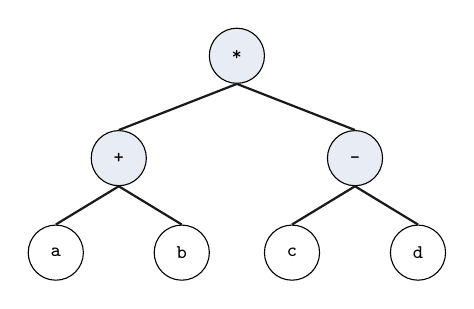
\begin{tikzpicture}[every node/.style={font=\scriptsize}]
    \node[draw, circle, minimum width=0.7cm, minimum height=0.7cm,
      fill=light-bg] (root) at (3.0, 2.5) {\texttt{*}};
    \node[draw, circle, minimum width=0.7cm, minimum height=0.7cm,
      fill=light-bg] (plus) at (1.5, 1.2) {\texttt{+}};
    \node[draw, circle, minimum width=0.7cm, minimum height=0.7cm,
      fill=light-bg] (minus) at (4.5, 1.2) {\texttt{-}};
    \node[draw, circle, minimum width=0.7cm, minimum height=0.7cm] (a) at (0.7, 0) {\texttt{a}};
    \node[draw, circle, minimum width=0.7cm, minimum height=0.7cm] (b) at (2.3, 0) {\texttt{b}};
    \node[draw, circle, minimum width=0.7cm, minimum height=0.7cm] (c) at (3.7, 0) {\texttt{c}};
    \node[draw, circle, minimum width=0.7cm, minimum height=0.7cm] (d) at (5.3, 0) {\texttt{d}};
    \draw[thick, color=jet] (root.south) -- (plus.north);
    \draw[thick, color=jet] (root.south) -- (minus.north);
    \draw[thick, color=jet] (plus.south) -- (a.north);
    \draw[thick, color=jet] (plus.south) -- (b.north);
    \draw[thick, color=jet] (minus.south) -- (c.north);
    \draw[thick, color=jet] (minus.south) -- (d.north);
  \end{tikzpicture}
  \caption{Expression tree for \texttt{*+ab-cd}: post-order reads \texttt{ab+cd-*}, pre-order reads \texttt{*+ab-cd}. Full story in Week~11.}
  \label{fig:exptree}
\end{figure}

\begin{example}[Prediction check: prefix \texttt{-+ab+cd} to postfix]
Of A: \texttt{ab+}, B: \texttt{cd+}, C: \texttt{ab+cd+-}, the first operator resolved is B --- \texttt{cd+}. Scanning right-to-left meets \texttt{d}, then \texttt{c}, both operands, and then the rightmost \texttt{+} with both its operands waiting --- so \texttt{d} and \texttt{c} combine under that \texttt{+} before anything else happens. A (\texttt{ab+}, the leftmost operator) resolves only after the scan reaches further left; C (the whole string at once) mistakes ``operators wait for both operands'' for ``everything waits'' --- in fact each operator fires the moment its own two operands are on top.
\end{example}

All three conversions cost one pass with each token pushed and popped at most once: $O(n)$ time worst case, $O(n)$ auxiliary space worst case, for $n$ tokens.

\section{Recursion and the Runtime Stack}

\textbf{Read alongside:} Karumanchi, Ch.~2, pp.62--73 (PDF) --- recursion, the call stack, recursion versus iteration; Wirth, \textit{Algorithms and Data Structures}, Ch.~3, pp.87--108 --- recursive algorithms, when recursion helps and when it does not.

\begin{definitionbox}{Recursive function}
A recursive function solves a smaller instance of its own problem: one \key{base case} answered directly, one \key{recursive case} that calls itself on strictly smaller input \cite{Karumanchi2017_data_structures_algorithms_made_easy,Wirth2004_algorithms_data_structures}.
\end{definitionbox}

The deck's canonical instance:
{\footnotesize
\begin{verbatim}
int fact(int n) {
    if (n <= 1) return 1;        /* base case */
    return n * fact(n - 1);      /* smaller instance */
}
\end{verbatim}
}
The \key{base case} (\texttt{n <= 1}, answered directly as $1$) stops the descent; the \key{recursive case} (\texttt{n * fact(n-1)}) shrinks the input by exactly one and trusts the smaller call's answer. Both halves are load-bearing. No base case: infinite descent, the stack filling until the program crashes. Input not shrinking: the same fate by a different road --- each call re-issues the same size and the chain never bottoms out.

\key{Iteration} keeps one frame and updates variables --- constant stack space, always explicit about progress. \key{Recursion} spends one frame per level --- the call chain \emph{is} the progress record, at $O(d)$ auxiliary space for depth $d$. Prefer recursion when the problem is self-similar (Hanoi, tree walks); prefer iteration when depth is large and the loop is simple (Wirth Ch.~3: when recursion does \emph{not} help). \muted{Same power, different ledger: recursion bills the runtime stack.}

\begin{definitionbox}{Frame (activation record)}
A \key{frame} holds one call's locals and its return address. Each call pushes a frame; each return pops it. Week~1's orientation holds: the stack grows down, the heap grows up.
\end{definitionbox}

Figure~\ref{fig:frames} shows four frames alive at once during \texttt{hanoi(3, S, D, A)}: \texttt{main} with \texttt{n = 3} at the bottom, then \texttt{hanoi(3, S, D, A)}, then \texttt{hanoi(2, S, A, D)}, with \texttt{hanoi(1, S, D, A)} running on top. The growth arrow points downward and the \texttt{top} label points at the running frame. Depth $d$ means $d$ frames alive --- Hanoi's depth is only $n$, but, as the next section prices, its calls number $2^{n}$.

\begin{figure}[h]
  \centering
  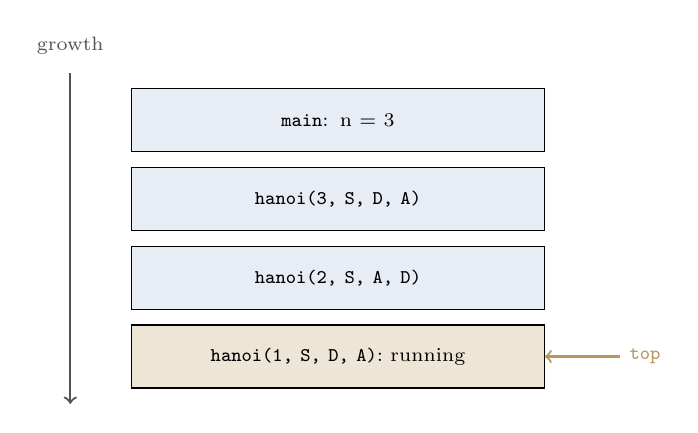
\begin{tikzpicture}[every node/.style={font=\scriptsize}]
    \node[draw, minimum width=5.2cm, minimum height=0.8cm, fill=light-bg,
      text width=5.0cm, align=center] (main) at (0, 0)
      {\texttt{main}: n = 3};
    \node[draw, minimum width=5.2cm, minimum height=0.8cm, fill=light-bg,
      text width=5.0cm, align=center] (h3) at (0, -1.0)
      {\texttt{hanoi(3, S, D, A)}};
    \node[draw, minimum width=5.2cm, minimum height=0.8cm, fill=light-bg,
      text width=5.0cm, align=center] (h2) at (0, -2.0)
      {\texttt{hanoi(2, S, A, D)}};
    \node[draw, minimum width=5.2cm, minimum height=0.8cm, fill=primary-gold!25,
      text width=5.0cm, align=center] (h1) at (0, -3.0)
      {\texttt{hanoi(1, S, D, A)}: running};
    \draw[->, thick, color=neutral] (-3.4, 0.6) -- (-3.4, -3.6);
    \node[text=neutral] at (-3.4, 0.95) {growth};
    \node[text=primary-gold] (toplab) at (3.9, -3.0) {\texttt{top}};
    \draw[->, thick, color=primary-gold] (toplab.west) -- (h1.east);
  \end{tikzpicture}
  \caption{Runtime-stack frames during Hanoi with $n = 3$: depth $4$ alive, \texttt{top} at the running call, growth downward.}
  \label{fig:frames}
\end{figure}

\section{Tower of Hanoi: Self-Similarity, Priced}

\textbf{Read alongside:} Karumanchi, Ch.~2, pp.62--73 (PDF) --- recurrence setup; Wirth, Ch.~3 --- recursive structure; Week~2 vocabulary for naming the operation, giving the bound, and stating the case.

Move the whole tower S $\to$ D; move one disk at a time; never place a larger disk on a smaller one. Figure~\ref{fig:hanoi} shows the start: three disks stacked on the source peg S, auxiliary peg A and destination peg D empty, the base line beneath and the peg labels below it. Three disks need 7 moves; $n$ disks need $2^{n} - 1$, proved below.

\begin{figure}[h]
  \centering
  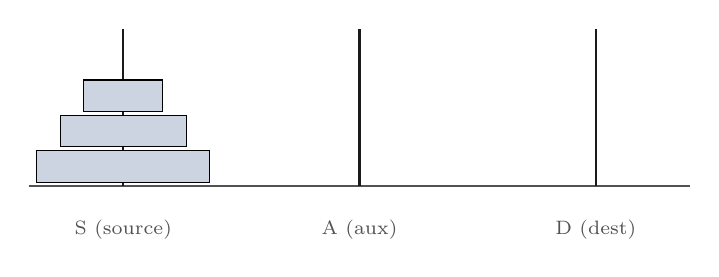
\begin{tikzpicture}[every node/.style={font=\scriptsize}]
    \draw[thick, color=neutral] (-1.2, 0) -- (7.2, 0);
    \draw[thick, color=jet] (0, 0) -- (0, 2.0);
    \draw[thick, color=jet] (3, 0) -- (3, 2.0);
    \draw[thick, color=jet] (6, 0) -- (6, 2.0);
    \node[draw, fill=primary-blue!20, minimum width=2.2cm,
      minimum height=0.4cm] (d3) at (0, 0.25) {};
    \node[draw, fill=primary-blue!20, minimum width=1.6cm,
      minimum height=0.4cm] (d2) at (0, 0.70) {};
    \node[draw, fill=primary-blue!20, minimum width=1.0cm,
      minimum height=0.4cm] (d1) at (0, 1.15) {};
    \node[text=neutral] at (0, -0.55) {S (source)};
    \node[text=neutral] at (3, -0.55) {A (aux)};
    \node[text=neutral] at (6, -0.55) {D (dest)};
  \end{tikzpicture}
  \caption{Tower of Hanoi, initial position with $n = 3$: the whole tower rests on S; A and D stand empty.}
  \label{fig:hanoi}
\end{figure}

\subsection{The recursive idea}

{\footnotesize
\begin{verbatim}
hanoi(n, src, dst, aux):
    if n == 1: move disk src -> dst
    else:
        hanoi(n-1, src, aux, dst)   /* park n-1 out of the way */
        move disk src -> dst        /* free the largest disk */
        hanoi(n-1, aux, dst, src)   /* stack the n-1 on top */
\end{verbatim}
}
The base case moves one disk. The recursive case reduces $n$ to $n - 1$ twice --- self-similarity made visible: park the top $n - 1$ disks on the spare peg, move the freed largest disk to its destination, then restack the $n - 1$ on top of it. Each ``move disk'' line is one counted step for the analysis next.

\begin{example}[Trace: three disks, seven moves]
Number the disks smallest, middle, largest, all starting on S. Move~1, smallest S $\to$ D: the small disk must vacate so the middle can move. Move~2, middle S $\to$ A: the middle parks on the spare peg. Move~3, smallest D $\to$ A: the small disk restacks on the middle, freeing both S and D. Move~4, largest S $\to$ D: the freed largest disk takes its destination --- the midpoint of the whole solution. Move~5, smallest A $\to$ S: the small disk vacates so the middle can move again. Move~6, middle A $\to$ D: the middle restacks on the largest. Move~7, smallest S $\to$ D: the small disk caps the tower. Moves~1--3 park two disks on A; move~4 frees the largest; moves~5--7 restack on D --- the algorithm above, executed line by line.
\end{example}

\subsection{Pricing Hanoi: \texorpdfstring{$T(n) = 2T(n-1) + 1$}{T(n) = 2T(n-1) + 1}}

Count disk moves, in Week~2's vocabulary. $T(1) = 1$; for $n > 1$, $T(n) = 2T(n-1) + 1$ (two sub-towers plus the largest disk's move). Unfold step by step. One level: $T(n) = 2T(n-1) + 1$. Two levels, substituting $T(n-1) = 2T(n-2) + 1$: $T(n) = 2(2T(n-2)+1) + 1 = 4T(n-2) + 3$. Three levels: $T(n) = 8T(n-3) + 7$. The pattern after $k$ levels is $T(n) = 2^{k}T(n-k) + (2^{k} - 1)$ --- each level doubles the pending subproblems and the accumulated $+1$s form $1 + 2 + 4 + \cdots + 2^{k-1} = 2^{k} - 1$. At $k = n - 1$ the recursion bottoms out: $T(n) = 2^{n-1} \cdot 1 + (2^{n-1} - 1) = 2^{n} - 1$. Hence $T(n) = 2^{n} - 1 = \Theta(2^{n})$ --- worst, best, and average coincide, because only one legal move sequence exists (at every non-trivial position exactly one move makes progress without undoing prior work). \key{Doubling the disks squares the work only in legend --- it multiplies the moves by roughly two per added disk, and $2^{64} - 1$ outlives us all.}

\subsection{What recursion bills you}

Three failure modes, each a way of misspending the runtime stack. \bad{Depth overflow}: $n = 100{,}000$ recursive frames burst the runtime stack --- the $O(d)$ ledger comes due, so iterate instead. \bad{Repeated subproblems}: naive recursive Fibonacci recomputes the same values exponentially often (each call re-solves what its siblings already solved) --- iteration or memoisation wins. \bad{Missing base case}: the stack fills until the program crashes --- the use-after-free of control flow, a frame leak with no return in sight. The habit, in Week~2's shape: name the operation (moves, frames), give the bound ($\Theta(2^{n})$ moves, $O(n)$ frames), state the case.

\begin{example}[Prediction check: Hanoi with $n = 4$]
Of A: 8 moves, 4 frames; B: 15 moves, 4 frames; C: 16 moves, 16 frames --- the answer is B. Moves: $2^{4} - 1 = 16 - 1 = 15$ (A doubles exactly instead of doubling-minus-one; C confuses $2^{n}$ with the move count). Frames: depth never exceeds $n$, so at most 4 frames are ever alive at once --- C mistakes total calls for simultaneous depth. \muted{Depth is the longest chain alive; moves count every call ever made.}
\end{example}

\section{Mistakes, Summary, and What Comes Next}

Three mistakes to retire now. \bad{Popping \texttt{\^{}} on a tie} --- right-associative means strictly-greater pops only; $a^{b^{c}}$ is not $(a^{b})^{c}$. \bad{Forgetting the paren swap on reversal} --- infix-to-prefix without swapping binds every bracket backwards. \bad{No base case, or input that never shrinks} --- Hanoi with \texttt{n-1} missing recurses until the stack bursts. The habit behind all three: trace the stack (operators, frames) line by line --- never from memory of the shape.

In summary: \key{Notations} --- infix for humans; postfix/prefix need no parens. \key{Conversions} --- infix to postfix (one left-to-right stack pass); infix to prefix (reverse, swap, postfix, reverse); prefix to postfix (right-to-left stack of strings) --- all $O(n)$ time worst case, $O(n)$ auxiliary space worst case. \key{Recursion} --- base plus shrinking self-call; frames on the runtime stack, $O(d)$ space for depth $d$. \key{Hanoi} --- $T(n) = 2T(n-1) + 1 = 2^{n} - 1 = \Theta(2^{n})$ moves; depth only $n$. Next week: queues --- what changes when the first element out is the first one in --- circular buffers, deques, and priority.

\subsection*{Exercises}

Answer from the algorithms, then check in the lab: both infix conversions are Lab P3, prefix to postfix is Lab P4.
\begin{enumerate}
  \item Postfix of \texttt{(a-b)*(c+d)}? Run the infix-to-postfix algorithm token by token and give the output and stack after each step.
  \item Prefix of \texttt{a+b*c}? Give it via the reverse--swap--postfix--reverse route, showing the reversed string and its postfix before the final reversal.
  \item Moves and max live frames for Hanoi $n = 5$? State both, naming the operation and the case for each bound.
  \item Convert \texttt{a+b*(c-d)/e} (this week's running example) to postfix with a full token trace. At which token does the first pop-to-output happen, and why?
  \item Convert prefix \texttt{+*ab*cd} to postfix by the right-to-left scan, showing the stack after every token. (Genuinely new instance reusing the deck's prefix-to-postfix rule.)
\end{enumerate}

\subsection*{Solutions}

\begingroup\small
\begin{enumerate}
  \item \textbf{Postfix \texttt{ab-cd+*}.} Trace: \texttt{(} pushes a marker; \texttt{a} appends (\texttt{a}); \texttt{-} pushes above the marker; \texttt{b} appends (\texttt{a b}); \texttt{)} flushes the \texttt{-} and discards the parens (\texttt{a b -}); \texttt{*} pushes; \texttt{(} pushes a second marker; \texttt{c} appends; \texttt{+} pushes above the marker; \texttt{d} appends; \texttt{)} flushes the \texttt{+} (\texttt{a b - c d +}); end of string pops the \texttt{*}: \texttt{ab-cd+*}. (The deck's own ``Before You Go'' answer, re-derived step by step.)
  \item \textbf{Prefix \texttt{+a*bc}.} Reverse \texttt{a+b*c} to \texttt{c*b+a}; postfix of the reversed string under the mirror rule is \texttt{cb*a+}; reverse back to \texttt{+a*bc}. Check outside-in: add $a$ to $\times(b,c)$ --- that is $a + b \times c$. Correct. (The deck's own ``Before You Go'' answer.)
  \item \textbf{$31$ moves, $5$ frames.} Moves: $T(5) = 2^{5} - 1 = 31$ disk moves (worst = best = average, one legal sequence). Frames: depth at most $n = 5$ live frames, $O(n)$ auxiliary space worst case. (The deck's own ``Before You Go'' answer.)
  \item \textbf{\texttt{abcd-*e/+}.} Trace: \texttt{a} appends; \texttt{+} pushes; \texttt{b} appends; \texttt{*} pushes above \texttt{+} (higher precedence, no pop); \texttt{(} pushes a marker; \texttt{c} appends; \texttt{-} pushes above the marker; \texttt{d} appends; \texttt{)} flushes \texttt{-} and discards the parens; \texttt{/} meets top \texttt{*} of equal precedence, left-associative, so it pops \texttt{*} first, then pushes \texttt{/}; \texttt{e} appends; end pops \texttt{/} then \texttt{+}. The first pop-to-output happens at \texttt{/}: it is the first operator that meets a waiting operator of equal-or-higher precedence (\texttt{*}), forcing the flush.
  \item \textbf{\texttt{ab*cd*+}.} Right to left: \texttt{d} pushes (\texttt{d}); \texttt{c} pushes (\texttt{d}, \texttt{c} with \texttt{c} on top); \texttt{*} pops \texttt{a} $=$ \texttt{c}, \texttt{b} $=$ \texttt{d}, pushes \texttt{cd*} (stack: \texttt{cd*}); \texttt{b} pushes (stack: \texttt{cd*}, \texttt{b}); \texttt{a} pushes (stack: \texttt{cd*}, \texttt{b}, \texttt{a}); \texttt{*} pops \texttt{a} $=$ \texttt{a}, \texttt{b} $=$ \texttt{b}, pushes \texttt{ab*} (stack: \texttt{cd*}, \texttt{ab*}); \texttt{+} pops \texttt{a} $=$ \texttt{ab*}, \texttt{b} $=$ \texttt{cd*}, pushes \texttt{ab*cd*+}. Outside-in check: add $\times(a,b)$ to $\times(c,d)$ --- the correct sum of products.
\end{enumerate}
\endgroup

\bibliography{../../Bibliography_base}
\bibliographystyle{plain}
\end{document}
